\chapter{Desarrollo} % Título del capítulo

\label{Desarrollo}

\section{Selección del microcontrolador}

\label{Selec}

Resulta imprescindible que el microcontrolador seleccionado para este proyecto de investigación cumpla con los siguientes requisitos:

%cambiar-listo!
\begin{itemize}
    \item Estar basado en una ISA RISC-V, ya que el contexto del proyecto está orientado a acoplar coprocesadores en núcleos RISC-V.
    \item Estar descrito en el lenguaje de descripción de hardware VHDL. 
En ocasiones, se han de modificar las fuentes del microcontrolador con el fin de acoplarle coprocesadores.
En este sentido, resulta más oportuno integrar todo en un mismo lenguaje. 
A pesar de que los sintetizadores soportan varios lenguajes, ciertos elementos pueden suponer incompatibilidades.
Por ejemplo, los tipos de datos varían dependiendo de cada lenguaje.
En consecuencia, se tendría que dedicar tiempo extra a realizar las adaptaciones necesarias.
Debido a que el coprocesador para aplicaciones de IA CRI está descrito en VHDL, se decide buscar un proyecto de microcontrolador descrito en este lenguaje.
    \item Contar con extensión de instrucciones para conectar coprocesadores mediante CFU, además de con soporte para comunicaciones mapeadas en memoria e interfaces \textit{stream}. 
Debido a que se necesita una variedad de métodos de conexión para realizar la caracterización del rendimiento, el microcontrolador seleccionado debe contar con al menos los mencionados.
\end{itemize} 

En este sentido, el NEORV32 \cite{gh:neorv32} cumple con todos estos requerimientos. 
Además, en la plataforma de desarrollo colaborativo donde está alojado, cuenta con una comunidad muy activa.
Es por ello que se encuentra bajo una revisión constante de fallos, tanto por parte del autor como de los usuarios.
De esta manera, se asegura en gran medida la correcta operatividad del mismo.
Además, el autor se dedica a realizar actualizaciones periódicas de sus funcionalidades.
Por si fuera poco, tanto el autor como la comunidad tienen una gran disponibilidad para responder dudas sobre temas relacionados con el proyecto, lo que resulta de gran ayuda.
Con respecto a la compilación de lenguajes de alto nivel, el proyecto ofrece \textit{toolchains} precompiladas de RISC-V para GCC.  
Estas herramientas permiten hacer compilación cruzada de C/C++ a instrucciones de RISC-V  en un entorno Linux \cite{gh:neorv32-tool}.
Cabe destacar que también se facilita un contenedor para realizar esta tarea \cite{gh:sim-conatiner}. 
Además, cuenta con un soporte de librerías para compilar funciones software específicas de NEORV32. 
Asimismo, el repositorio ofrece una variedad de ejemplos de aplicación software de todos los recursos con los que cuenta el micro.
Además de todo lo mencionado, este microcontrolador cuenta con una hoja de características \cite{neorv32-ds} y una guía de usuario \cite{neorv32-ug} realizadas por el autor y actualizadas a la par que el código del proyecto, las cuales destacan por su calidad.
Teniendo en cuenta todas estas consideraciones, el NEORV32 es el procesador seleccionado para este proyecto.

\section{Flujo de trabajo}

\label{Workf}

Las herramientas EDA FLOS y las propietarias/comerciales no son ecosistemas aislados.
Al contrario, en los últimos años se han visto colaboraciones de proyectos \textit{Open Source} con iniciativas privativas.
En este sentido, se puede destacar la integración de la herramienta RapidWright \cite{gh:rapid} a la \textit{Suite} de diseño Vivado.
En concreto, este proyeto \textit{Open Source} desarrollado por \textit{AMD Research and Advanced Development} tiene como objetivo permitir a los usuarios avanzados una mayor flexibilidad a la hora de personalizar sus soluciones mediante una metodología de diseño utilizando módulos pre-implementados.
Además, se han realizado concursos \cite{contest} patrocinados por AMD con el objetivo de promover y demostrar que el \textit{FPGA Interchange Format} (FPGAIF - Formato de Intercambio de FPGA) \cite{FPGAIF} es una representación intermediaria eficiente y robusta para trabajar en problemas de \textit{backends} de FPGAs, incluso a escala industrial.
Asimismo, este tipo de iniciativas también tratan de fomentar la innovación de algoritmos de enrutamiento de FPGAs que den prioridad al tiempo de ejecución, con objeto de posibilitar su aplicación en la emulación de ASICs.
Cabe destacar que el FPGAIF es un estándar de formato de intercambio diseñado para proporcionar toda la información necesaria mediante la cual realizar el \textit{place and route} en un contexto \textit{Open Source}.
En la misma línea, Siemens ha observado un crecimiento saludable entorno a la \textit{Open Source VHDL Verification Methodology} (OSVVM - Metodología de Verificación VHDL de Código Abierto) \cite{osvvm} y la \textit{Universal VHDL Verification Methodology} (UVVM -  Metodología de Verificación Universal VHDL) \cite{uvvm} desde 2018, lo que en sus propias palabras \say{es alentador} \cite{wilson-research}.
Por lo tanto, a la vista de estos ejemplos, podemos afirmar que los comerciales tradicionales de herramientas EDA están empezando a facilitar el uso de herramientas FLOS e incluso a integrar parte o la totalidad de las mismas en sus propuestas comerciales.
Este hecho refleja un futuro híbrido en lo referente al ecosistema de herramientas para FPGAs.

\begin{figure}[h!]
    \centering
    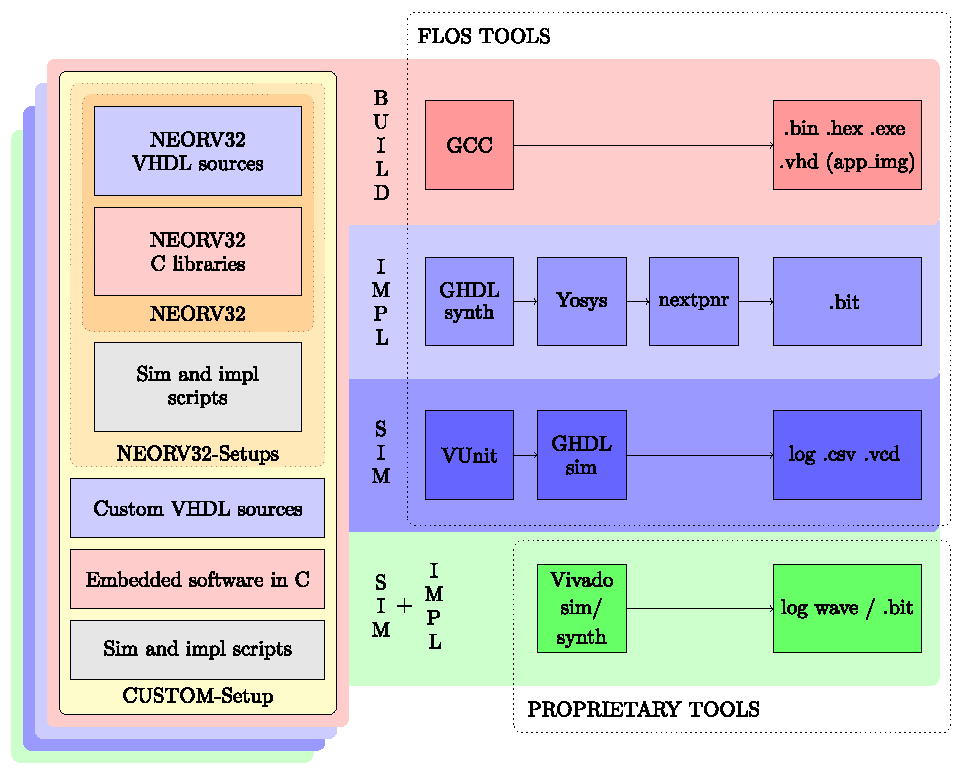
\includegraphics[width=14cm]{Figuras/workflow.pdf}
    \caption{\textit{Workflow} del \textit{Setup} personalizado.}
    \label{fig:workf}
\end{figure}

Atendiendo a este nuevo paradigma híbrido de herramientas, en el presente trabajo de investigación se propone el uso tanto de herramientas FLOS como privativas.
Como se observa en la figura \ref{fig:workf}, el flujo de trabajo propuesto es el siguiente:

\begin{itemize}
    \item \textbf{Compilación}: respecto a la compilación cruzada de software en C, de x86 (64 bits) a RISC-V (32 bits), se emplea la herramienta FLOS GCC.
    \item \textbf{Implementación}: respecto a las implementaciones en placa de los diseños, se efectúan mediante dos vías paralelas:
        \begin{itemize}
            \item Haciendo uso del conjunto de herramientas FLOS: GHDL \cite{gh:ghdl}, yosys \cite{gh:yosys}, GHDL yosys plugin \cite{gh:ghdl-plugin}, nextpnr-xilinx \cite{gh:nextpnr} y prjxray \cite{gh:prjxray} para realizar la elaboración, la síntesis y el \textit{place and route} y de la herramienta openFPGALoader \cite{gh:openFPGALoader} para cargar el \textit{bitstream} en la placa.
            \item Haciendo uso de la \textit{Suite} de diseño privativa Vivado.
        \end{itemize}
Esto se debe a que la generación automática de \textit{bitstreams} mediante la integración continua de repositorios públicos está limitada al uso de herramientas FLOS.
Asimismo, la implementación más eficiente de los diseños, en términos de gestión de recursos de la Arty, está condicionada al uso de herramientas privativas.
Por ello, se eligen la generación mediante ambas vías.
Además, para realizar una verificación doblemente redundante, se implementa tanto en la Arty A7 35T como en la 100T.
    \item \textbf{Simulación}: respecto a las simulaciones realizadas a lo largo de las secciones \ref{Carac} y \ref{Integ} se emplea principalmente el \textit{framework} FLOS VUnit \cite{gh:vunit}, con el cual se realizan todas ellas.
No obstante, también se utiliza Vivado en ciertas ocasiones.  
En concreto, en los ensayos en los que se hace uso de la funcionalidad ILA.
Esta funcionalidad se ha utilizado, por ejemplo, para testear la correcta operatividad de un \textit{wrapper} Wishbone.
\end{itemize} 

Las herramientas descritas en la explicación de este flujo de trabajo no solo se utilizan a nivel local, sino que también se emplean, todas o parte de ellas, en la \textbf{integración continua (CI)} de repositorios \textit{online}, tanto en el GitLab del grupo de investigación como en el GitHub propio.
Para ello, se utilizan varios \textbf{contenedores}.
Para la generación de \textit{bitstream} mediante herramientas FLOS, se utiliza el contenedor mencionado en la sección \ref{ben}, el cual es generado a su vez en CI.
Este contenedor se utiliza en la integración continua tanto del repositorio de GitLab como de GitHub.
Para la generación de \textit{bitstream} mediante Vivado, se utiliza una contenedor que solamente es accesible por los ordenadores del laboratorio del grupo de investigación, el cual está alojado en nuestro servidor Orion.
Esto es debido a que al ser un programa privativo no se pueden distribuir publicamente contenedores con este software. A consecuencia de ello, la generación de \textit{bitstream} mediante esta vía solo está disponible en la integración continua del repositorio del grupo (GitLab).
Para realizar los ensayos en simulación, se utilizan principalmente dos contenedores de VUnit.
El \href{https://console.cloud.google.com/gcr/images/hdl-containers/global/sim/osvb}{gcr.io/hdl-containers/sim/osvb:latest} con GHDL compilado con llvm como \textit{backend} y el \href{https://hub.docker.com/layers/ghdl/vunit/mcode-master/images/sha256-e32029c5be70a5fa0fc94bffd15d72fa8b84ad8aaf2dc7cfa8ab8324ef733ed0?context=explore}{docker.io/ghdl/vunit:mcode-master} con GHDL compilado con mcode como \textit{backend}.
Esto se debe a que la funcionalidad \href{https://github.com/stnolting/neorv32/discussions/886}{\textit{external names}}, para capturar señales de jerarquías inferiores, solo es soportada en GHDL si este está compilado con el \textit{backend} mcode.
En definitiva, el uso de estos recursos mediante la metodología de integración continua posibilita automatizar todas las simulaciones, visualizando y gestionando sus resultados, así como la generación de todos los \textit{bitstreams}, cada vez que se hace un \textit{push} al repositorio.
Cabe destacar que la compilación de software solo se realiza en local, aunque también se utiliza un contenedor \cite{gh:sim-conatiner}, no está automatizada en integración continua.

\subsection{Cargar software en el NEORV32}

Antes de entrar en los detalles del acoplamiento de periféricos \textit{custom}, se procede a realizar un repaso de cómo cargar un software en C al \textit{softcore} NEORV32.
Como se ha mencionado, el proyecto NEORV32 proporciona \textit{toolchains} de RISC-V para GCC con las que realizar la compilación cruzada desde Linux a la arquitectura RISC-V.
Estas herramientas están acompañadas de archivos \textit{Makefiles} mediante los cuales se permiten añadir argumentos al comando \textit{Make}, con objeto de, entre otras cosas, proporcionar el programa compilado en diferentes formatos de salida.
A lo largo de esta sección, nos centraremos en tres de estos formatos:

\begin{itemize}
    \item Ejecutable, \textit{exe} (.bin)
    \item app\_image (.vhd)
    \item Hexadecimal (.hex)
\end{itemize} 

Cada una de estas salidas tiene la misma información, el programa compilado.
No obstante, cada una de ellas puede utilizarse para cargar el software en la IMEM (memoria de instrucciones) en diferentes puntos del flujo de trabajo:

\begin{itemize}
    \item El \textit{exe} se puede cargar en el NEORV32 una vez que esté ejecutándose en la FPGA. Esta transferencia se realiza a través del \textit{bootloader}.
    \item La app\_image remplaza el contenido por defecto de una de las fuentes RTL del diseño del NEORV32, de modo que su contenido se codifica cuando este se sintetiza.
    \item El archivo .hex se lee durante la síntesis, por lo que es equivalente a la solución de la app\_image, pero no requiere modificar las fuentes RTL cada vez que se actualiza el software a cargar.
\end{itemize} 

Estas opciones se resumen en la tabla \ref{tab:2}.

\begin{table}[h!]
\centering
\caption{Tres formas de introducir software en la IMEM.}
\label{tab:2}
\begin{tabular}{|c|c|c|c|}
\hline
\textbf{Formato}  & \textbf{Comando}   & \textbf{Descripción}                                                                                            & \textbf{Bootloader}  \\ \hline
.bin              & make exe           & \begin{tabular}[c]{@{}c@{}}Después de la implementación,\\  cargar el exe mediante la CMD\end{tabular}          & Habilitado           \\ \hline
.vhd              & make image         & \begin{tabular}[c]{@{}c@{}}Antes de la síntesis, \\ sustituir la app\_image por defecto\end{tabular}            & Deshabilitado        \\ \hline
.hex              & make hex           & Durante la síntesis, leer del .hex                                                                              & Deshabilitado        \\ \hline
\end{tabular}
\end{table}

\subsubsection{\textit{Bootloader}}
\label{boot}

El NEORV32 viene por defecto con un \textit{bootloader} que se encarga de establecer la comunicación serie vía UART y generar una CMD visible desde terminales como CuteCom \cite{gh:cutecom}, \href{https://man.openbsd.org/cu.1}{cu}, o \href{https://www.gnu.org/software/screen/}{screen} en GNU/Linux.
En este sentido, hay tres formas posibles de proceder:

\begin{itemize}
    \item Deshabilitar el \textit{bootloader} y cargar/iniciar un programa desde la app\_image o desde un archivo hexadecimal.
        \begin{itemize}
            \item No se utiliza el \textit{bootloader}.
        \end{itemize} 
    \item Habilitar el \textit{bootloader} y cargar/iniciar un programa a través del \textit{Autoboot}.
        \begin{itemize}
            \item Después del \textit{reset}, cuando el \textit{bootloader} está habilitado, la primera secuencia que ocurre es el \textit{Autoboot}. 
Esta secuencia intenta obtener una imagen de arranque válida desde la flash SPI externa.
Si se encuentra una imagen válida que se pueda transferir correctamente a la IMEM (memoria de instrucciones), se inicia automáticamente la aplicación.
No obstante, si han pasado 8 segundos y no se ha detectado ninguna flash SPI o no se encuentra ninguna imagen de arranque válida, se mostrará el código de error \say{ERR EXE}, bloqueando la ejecución.
Sin embargo, durante esos 8 segundos, se puede detener la secuencia del \textit{Autoboot} pulsando cualquier tecla. 
De esta manera, se pone a disposición una CMD lista para recibir comandos.
        \end{itemize} 
    \item Habilitar el \textit{bootloader} y cargar/iniciar un programa a través de comandos en la CMD.
Los comandos soportados son los siguientes:
        \begin{itemize}
            \item \say{h} - Muestra el texto de ayuda.
            \item \say{r} - Reiniciar el \textit{bootloader}.
            \item \say{u} - Cargar un programa en formato ejecutable (\textit{neorv32\_exe.bin}) a la IMEM.
            \item \say{s} - Almacenar un ejecutable en flash SPI.
            \item \say{l} - Cargar un ejecutable desde flash SPI.
            \item \say{x} - Arrancar un programa desde flash a través de XIP.
            \item \say{e} - Iniciar un programa almacenado en la IMEM.
        \end{itemize} 
\end{itemize} 

Para elegir una de estas tres formas de proceder, se debe entender que el \textit{bootloader} es útil/necesario cuando:

    \begin{itemize}
        \item La FPGA utilizada no permite inicializar la memoria en el \textit{bitstream}. 
En consecuencia, no es posible cargar/arrancar programas a través de la app\_image.
Este es el caso de las FPGAs con SPRAM, como la Lattice ICE40 (UP3K, UP5K).
        \item Múltiples programas deben ser cargados/arrancados durante el desarrollo, sin resintetizar el diseño.
    \end{itemize} 

En la figura \ref{fig:boot} se muestra como cargar/iniciar un programa ejecutable (.exe) al NEORV32 mediante la CMD proporcionada por el \textit{bootloader}. 
Concretamente, se utiliza la terminal CuteCom \footnote {En CuteCom, el archivo que se carga a la terminal debe ser de tipo \textit{Plain} (como se muestra en la figura \ref{fig:boot}), de lo contrario se dará el error \say{ERR EXE}.}, en ella se emplean sucesivamente los comandos \say{u} (\textit{upload} - cargar) y \say{e} (\textit{execute} - ejecutar).

\begin{figure}[h!]
    \centering
    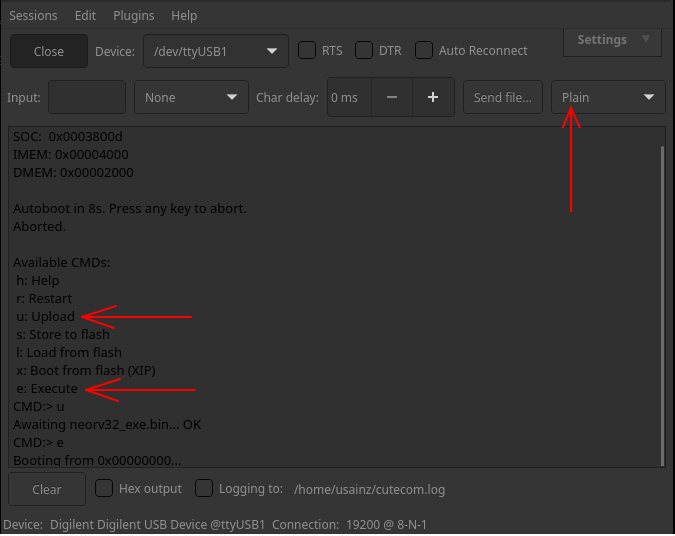
\includegraphics[width=14cm]{Figuras/cutecom_cmd_upload.png}
    \caption{Cargar un \textit{exe} a través del \textit{bootloader} de NEORV32 (terminal CuteCom).}
    \label{fig:boot}
\end{figure}

\subsubsection{Habilitar/Deshabilitar el \textit{Bootloader}}

Si el \textit{bootloader} no es útil/necesario para nuestra aplicación tendremos que considerar lo siguiente.
La IMEM se puede implementar de dos formas, como una RAM vacía o como una ROM inicializada a través del archivo que contiene el programa compilado, ya sea la \textit{neorv32\_application\_image.vhd} o el hexadecimal. 
Con el genérico \mintinline[breaklines]{vhdl}{IMEM_AS_IROM} se selecciona la implementación de la IMEM mediante una de estas dos opciones. 
Este genérico es
 
\hspace{35mm} \mintinline[breaklines]{vhdl}{IMEM_AS_IROM => imem_as_rom_c} 

\noindent y se define como 

\hspace{17mm} \mintinline[breaklines]{vhdl}{imem_as_rom_c : boolean := not INT_BOOTLOADER_EN;}

\noindent Por lo tanto, para cargar un programa desde la \textit{neorv32\_application\_image.vhd} (o desde el hexadecimal), la IMEM debe implementarse como una ROM inicializada mediante ese archivo, por lo que el \textit{bootloader} \textbf{debe estar deshabilitado}.
Se discutió con Stephan \href{https://github.com/stnolting/neorv32/discussions/824}{(\#824)} acerca de por qué la IMEM se inicializa como una RAM vacía cuando el \textit{bootloader} está activado. 
Y según el diseñador del NEORV32, \say{si la IMEM se implementara como una RAM preinicializada, entonces la imagen podría corromperse durante el tiempo de ejecución (imagina algún puntero deshonesto escribiendo en la IMEM), lo que requeriría volver a cargar el programa original. 
Por lo tanto, la carga del \textit{bootloader} se requeriría de todos modos.}

El proceso para deshabilitar el \textit{bootloader} es sencillo, en el TOP del diseño del NEORV32, se debe cambiar la constante \mintinline[breaklines]{vhdl}{INT_BOOTLOADER_EN} de \textit{true} a \textit{false}, como se muestra en el extracto de código \ref{code:1}.

\begin{code}
\begin{minted}[frame=lines,framesep=2mm,baselinestretch=1.2,fontsize=\footnotesize]{vhdl}
neorv32_top_inst : neorv32_top
generic map(
----------------------------------
INT_BOOTLOADER_EN         => false,
----------------------------------
)
\end{minted}
\caption{Constante para deshabilitar el \textit{bootloader}.}
\label{code:1}
\end{code}

\subsubsection{Cargar un programa compilado desde un archivo hexadecimal}

Como se ha mencionado, en vez de cargar un programa compilado desde el archivo \textit{neorv32\_application\_image.vhd}, es posible cargar el programa compilado desde un archivo hexadecimal (.hex).
Para ello, se necesitan hacer unas pequeñas modificaciones en el código HDL del NEORV32.
En particular, se debe añadir una nueva función en el paquete \textit{neorve32\_package.vhd}.
Esta función se encargará de leer el archivo hexadecimal usando la librería \textit{std.textio.all}. \footnote{Esta librería está soportada desde la versión VHDL 2008.}
La función en cuestión es la descrita en el extracto de código \ref{code:2}.

\begin{code}
\begin{minted}[frame=lines,framesep=2mm,baselinestretch=1.2,fontsize=\footnotesize]{vhdl}
-- Initialize mem32_t from hex
-- MEMORY_SIZE is IMEM_SIZE/4, see neorv32_imem.default.vhd

impure function mem32_init_hex(name : STRING; MEMORY_SIZE : natural) return mem32_t is
    file rom_file : text open read_mode is name;
    variable rom_line : line;
    variable temp_word : std_ulogic_vector(31 downto 0);
    variable temp_rom : mem32_t(0 to MEMORY_SIZE-1) := (others => (others => '0'));
begin
    for i in 0 to MEMORY_SIZE - 1 loop
        exit when endfile(rom_file);
        readline(rom_file, rom_line);
        hread(rom_line, temp_word);
        temp_rom(i) := temp_word;
    end loop;

    return temp_rom;
end function;
\end{minted}
\caption{Función a añadir al \textit{neorve32\_package.vhd} para leer un software compilado en formato hexadecimal.}
\label{code:2}
\end{code}

Además, se debe modificar el archivo \textit{neorv32\_imem.default.vhd} \footnote{En el archivo \textit{neorv32\_imem.default.vhd} se debe comentar el código relacionado con cargar la ROM desde la app\_image.} para cargar el contenido del archivo hexadecimal (\textit{neorv32\_raw\_exe.hex}) a la memoria de instrucciones, usando la función definida en el extracto de código \ref{code:2}.
Para ello se debe añadir el extracto de código \ref{code:3}.

\begin{code}
\begin{minted}[frame=lines,framesep=2mm,baselinestretch=1.2,fontsize=\footnotesize]{vhdl}
constant ROM_INIT_FILE : string := "neorv32_raw_exe.hex";
-- ROM - initialized with hex code --
constant mem_rom_c : mem32_t(0 to IMEM_SIZE/4-1) := mem32_init_hex(ROM_INIT_FILE, 
IMEM_SIZE/4);
\end{minted}
\caption{Modificación del archivo \textit{neorv32\_imem.default.vhd} para cargar la IMEM mediante la función descrita en el extracto de código \ref{code:2}.}
\label{code:3}
\end{code}

Este método propone leer desde VHDL un formato hexadecimal, el cual es una salida nativa del compilador, en lugar de autogenerar código HDL con el programa compilado como pasa cuando utilizamos la opción de la app\_image. 
Ambas opciones cargan la IMEM cuando se sintetiza el diseño.
Sin embargo, con la opción de lectura del archivo .hex conseguimos dos cosas: no autogenerar código HDL tras la compilación y no modificar el código HDL existente cada vez que se actualiza el software a cargar.

Por último, cabe destacar que a lo largo del desarrollo de este proyecto se ha cargado software compilado al NEORV32 mediante los tres formatos expuestos.
No obstante, mayoritariamente se ha utilizado el formato .vhd generando una \textit{neorv32   \_application\_image.vhd} para cada software empleado.

\section{Caracterización del rendimiento de los métodos de conexión}

\label{Carac}

%Se han hecho x ensayos relatarlos, x implementaciones. 

Para caracterizar el rendimiento de los diferentes modos de conexión con los que cuenta el NEORV32, se propone acoplarle 3 tipos de multiplicadores con diferentes características.
Debido a que el objetivo de esta sección es caracterizar los métodos de acoplamiento, no son relevantes las funciones del coprocesador en sí. 
En este sentido, se ha pretendido emular en ellos cualidades de rendimiento y tiempo de respuesta propias de coprocesadores de IA.
Para ello, se han establecido ciertos patrones que comparten los aceleradores que se pretenden integrar en aplicaciones futuras, ver \ref{lin-fut}.
De esta manera, se ha determinado que las características de almacenamiento a la entrada/salida, así como de segmentación de señales internas, son cualidades a imitar.
Además, se decide realizar dos tipos de ensayos, con objeto de evaluar los métodos de conexión en términos de latencia y \textit{throughput}.
Cabe destacar que para el caso de los métodos \textit{Stream Link Interface} (SLINK) y \textit{Processor-External Bus Interface} (XBUS), se realiza una caracterización adicional acoplando los 3 multiplicadores a \textit{Verification Components}\footnote{Herramienta de verificación funcional que ofrece el \textit{framework} VUnit.} de AXI-Stream y Wishbone respectivamente.
De esta manera, se realiza por cada multiplicador acoplado mediante cada método de conexión un ensayo de latencia y si es posible de \textit{throughput}.
Esto es debido a que para realizar una caracterización de \textit{throughput}, el acelerador o el modo de conexión debe disponer de un \textit{buffer} de datos.
Teniendo en cuenta estas consideraciones, se han llevado a cabo un total de 29 ensayos de simulación con éxito, todos ellos realizados mediante el \textit{framework} VUnit.
Dichos ensayos se resumen en la tabla \ref{tab:3}.
Asimismo, se han implementado en FPGA todos los diseños realizados referentes al conjunto NEORV32 más multiplicador, con objeto de verificar en placa su correcta operatividad.

\begin{table}[h!]
\centering
\caption{Ensayos de latencia y \textit{throughput} realizados: VC, el multiplicador solo acoplado a \textit{Verification Components}; C, el SoC completo incluyendo el NEORV32, el multiplicador y la ejecución de software.}
\label{tab:3}
\begin{tabular}{|cl|cc|cc|c|c|}
\hline
\multicolumn{2}{|c|}{\multirow{2}{*}{\diagbox[]{\textbf{Tipo}}{\textbf{Modo}}}} & \multicolumn{2}{c|}{\textbf{SLINK}}           & \multicolumn{2}{c|}{\textbf{XBUS}}            & \textbf{CFU} & \textbf{CFS} \\ \cline{3-8} 
\multicolumn{2}{|c|}{}                                                          & \multicolumn{1}{c|}{\textbf{VC}} & \textbf{C} & \multicolumn{1}{c|}{\textbf{VC}} & \textbf{C} & \textbf{C}   & \textbf{C}   \\ \hline
\multicolumn{2}{|c|}{\textbf{Mult-B}}                                           & \multicolumn{1}{c|}{Ambos\tablefootnote{\say{Ambos} se refiere a que se han realizado los ensayos tanto de latencia como de \textit{throughput}.}}       & Ambos      & \multicolumn{1}{c|}{Ambos}       & Ambos      & Latencia     & Ambos        \\ \hline
\multicolumn{2}{|c|}{\textbf{Mult-BP}}                                          & \multicolumn{1}{c|}{Ambos}       & Ambos      & \multicolumn{1}{c|}{Ambos}       & Ambos      & Latencia     & Ambos        \\ \hline
\multicolumn{2}{|c|}{\textbf{Mult-UBP}}                                         & \multicolumn{1}{c|}{Latencia}    & Ambos      & \multicolumn{1}{c|}{Latencia}    & Latencia   & Latencia     & Latencia     \\ \hline
\end{tabular}
\end{table}

\subsection{Descripción y conexión de los multiplicadores}

\label{decrip}

%descripcion de los multiplicadores las funciones utilizadas

\begin{figure}[h!]
    \centering
    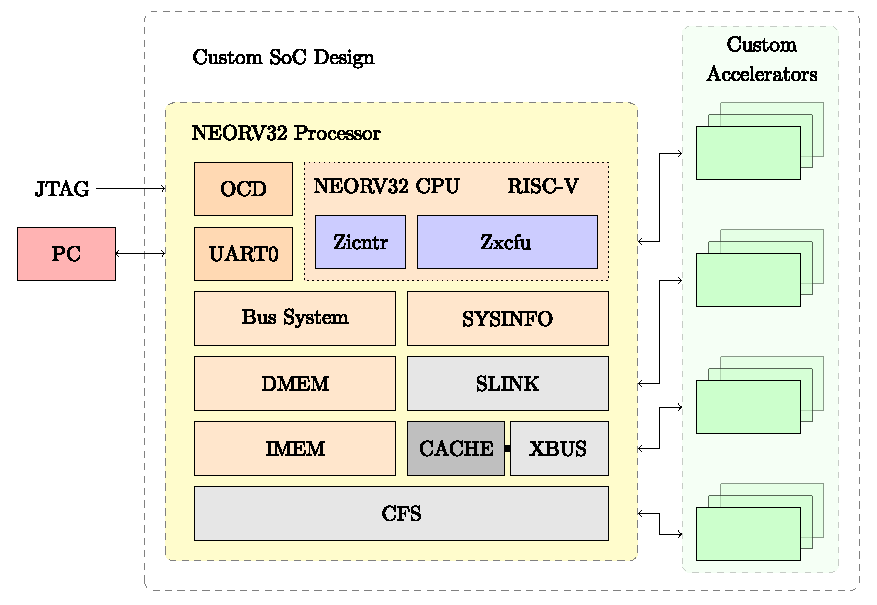
\includegraphics[width=14cm]{Figuras/scheme.pdf}
    \caption{Esquema de las posibles combinaciones del SoC personalizado.}
    \label{fig:soc}
\end{figure}

La figura \ref{fig:soc} ilustra las posibles combinaciones de acoplamiento de los 3 diferentes multiplicadores mediante los modos de conexión SLINK, XBUS, CFU y CFS.
Las características que definen a cada tipo de multiplicador son las siguientes:

\begin{itemize}
    \item \textbf{Mult-B} (\textbf{Mult}iplicador\textit{\textbf{-B}uffered}), en el código HDL del proyecto referido como \textit{Mult\_wfifos}, es un multiplicador al que se le han añadido dos FIFOs, una a la entrada y otra a la salida.
Además, las señales internas se gestionan mediante una máquina de estados. 
Es configurable en número de bits de entrada/salida y en profundidad de la FIFO, aunque normalmente se ha configurado en 32 y 4 bits respectivamente.
Puede recibir hasta tres relojes diferentes, uno en la FIFO de entrada, otro en el multiplicador y otro en la FIFO de salida, aunque comúnmente se han ajustado los tres la misma frecuencia.
Su topología interna se puede observar en el apéndice \ref{Planos}, plano \ref{fig:mult-b}.
Además, su descripción hardware se encuentra en el apéndice \ref{Codigo}, código \ref{ap-cod:3}.
\item \textbf{Mult-BP} (\textbf{Mult}iplicador\textit{\textbf{-B}uffered} y \textit{\textbf{P}ipelined}), en el código HDL del proyecto referido como \textit{Multp\_wfifos}, es un multiplicador al que se le han añadido dos FIFOs, una a la entrada y otra a la salida, pero al contrario que Mult-B, las señales internas se gestionan segmentadas.
Es configurable en número de bits de entrada/salida y en profundidad de la FIFO, aunque normalmente se ha configurado en 32 y 4 bits respectivamente.
Puede recibir hasta tres relojes diferentes, uno en la FIFO de entrada, otro en el multiplicador y otro en la FIFO de salida, aunque comúnmente se han ajustado a la misma frecuencia.
Cabe destacar que su descripción hardware se encuentra en el apéndice \ref{Codigo}, código \ref{ap-cod:7}.
\item \textbf{Mult-UBP} (\textbf{Mult}iplicador\textit{\textbf{-U}n\textbf{B}uffered} y \textit{\textbf{P}ipelined}), en el código HDL del proyecto referido como \textit{Multp}, es un multiplicador sin \textit{buffers} de entrada/salida, además las señales internas se gestionan segmentadas.
Es configurable en número de bits de entrada/salida, aunque normalmente se ha configurado en 32 bits.
Cabe destacar que su descripción hardware se encuentra en el apéndice \ref{Codigo}, código \ref{ap-cod:6}.
\end{itemize}

Para realizar el acoplamiento de los multiplicadores con las interfaces SLINK (AXI-Stream) y XBUS (Wishbone), se han realizado \textit{wrappers} definidos en el apéndice \ref{Codigo}.
En concreto, para el caso del Mult-B la descripción HDL del \textit{wrapper} se encuentra en el código \ref{ap-cod:4} y \ref{ap-cod:5}, para AXI y Wishbone respectivamente.
Para el caso del Mult-BP, en el código \ref{ap-cod:8} y \ref{ap-cod:9}, para AXI y Wishbone respectivamente.
Para el caso del Mult-UBP las señales AXI estan autocontenidas en la descripción de su diseño \ref{ap-cod:6}, así como el \textit{wrapper} para Wishbone está descrito en \ref{ap-cod:10}.

En lo que respecta al software, se han empleado funciones de C propias del NEORV32 para interactuar con cada uno de los modos de conexión.
Mediante las librerías aportadas por Stephan, tras compilarse, estas funciones se transforman a instrucciones interpretables por RISC-V.
Dichas funciones son las siguientes:
\begin{itemize}
    \item SLINK:
        \begin{itemize}
            \item Para enviar datos del NEORV32 al coprocesador: \mintinline[bgcolor=pink,breaklines]{c}{neorv32_slink_put(dato)} 
            \item Para recibir datos del coprocesador al NEORV32: \mintinline[bgcolor=pink,breaklines]{c}{neorv32_slink_get()} 
        \end{itemize}
    \item XBUS:
        \begin{itemize}
            \item Para enviar datos del NEORV32 al coprocesador: \mintinline[bgcolor=pink,breaklines]{c}{neorv32_cpu_store_}    \mintinline[bgcolor=pink,breaklines]{c}{unsigned_word(dirección,dato)} 
            \item Para recibir datos del coprocesador al NEORV32: \mintinline[bgcolor=pink,breaklines]{c}{neorv32_cpu_load_}   \mintinline[bgcolor=pink,breaklines]{c}{unsigned_word(dirección)} 
        \end{itemize}
    \item CFU:
        \begin{itemize}
            \item Para enviar datos del NEORV32 al coprocesador y recibir, en función de dichos datos, la salida del coprocesador en la misma ejecución de la instrucción: \mintinline[bgcolor=pink,breaklines]{c}{neorv32_cfu_r3_instr(funct7,funct3, rs1, rs2)} 
        \end{itemize}
    \item CFS:
        \begin{itemize}
            \item Para enviar datos del NEORV32 al registro mapeado en memoria con el coprocesador: \mintinline[bgcolor=pink,breaklines]{c}{NEORV32_CFS->REG[0] = dato_de_salida;} \footnote{Los registros disponibles asociados a CFS son del REG[0] al REG[63].}
            \item Para recibir datos del registro mapeado en memoria con el coprocesador al NEORV32: \mintinline[bgcolor=pink,breaklines]{c}{dato_de_entrada = NEORV32_CFS->REG[0];} 
        \end{itemize}
\end{itemize}

En este sentido, en el apéndice \ref{Codigo} se muestran los programas en C realizados para llevar a cabo los diferentes métodos de conexión.
Se observa que en todos ellos se emplea un \mintinline[breaklines]{c}{#ifdef}.
El objetivo de esto es separar la compilación de software orientado a ser simulado, con muy pocos \mintinline[breaklines]{c}{printf} para agilizar la simulación y la del software orientado a ser implementado en FPGA.
En concreto, en el código \ref{ap-cod:11} se muestra el main.c para SLINK, en \ref{ap-cod:12} para XBUS, en \ref{ap-cod:13} para CFU y en \ref{ap-cod:14} y \ref{ap-cod:15} para CFS.
Respecto a este último, se realiza esta división porque el primer programa está orientado a multiplicadores \textit{buffered} y el segundo al \textit{unbuffered}.
Esto es debido a que para el primer caso, se destina un registro mapeado en memoria para gestionar las señales de lectura/escritura, además de otro registro para las entradas/salidas. No obstante, para el caso del multiplicador \textit{unbuffered} solo se necesita un registro para gestionar las entradas/salidas, por lo que el software varía.
Cabe destacar que se genera una app\_image por cada programa compilado, teniendo en cuenta que los \mintinline[breaklines]{c}{#define} se van comentando para obtener un programa destinado a simulación, de latencia o throughput o a implementación.

Con respecto a la CFU, se realiza una instrucción \textit{custom} para operar cada multiplicador.
En concreto, se utilizan tres instrucciones \textit{R3-Type} de la extensión Zxcfu.
Se emplea el registro \textit{rs1} para la entrada de la multiplicación, los 16 primeros bits para el primer factor y los 16 últimos para el segundo.
El segundo registro fuente \textit{rs2} no se utiliza y el resultado de la multiplicación se guarda en el registro de destino \textit{rd}.
Para especificar la instrucción de cada multiplicador se emplea el campo \textit{funct3}, también se puede emplear el campo \textit{funct7} pero en este caso no se tiene en cuenta.
En concreto, \mintinline[breaklines]{c}{funct3=000} se asocia a Mult-B, \mintinline[breaklines]{c}{funct3=001} a Mult-BP y \mintinline[breaklines]{c}{funct3=010} a Mult-UBP.
En el código \ref{ap-cod:16}, se observa cómo están integrados los multiplicadores en el \textit{core} del NEORV32.
Además, se aprecia cómo se evalúa el campo \textit{funct3} para dirigir la información de entrada/salida a cada uno de los multiplicadores, así como se observan los recursos lógicos empleados para iniciar las operaciones e indicar cuándo estas han terminado.

Con respecto al subsistema CFS, como se ha mencionado, se distinguen dos casos. 
Por un lado, para el caso de los multiplicadores \textit{buffered}, se mapean 2 de los 64 registros asociados, el registro REG[0] para los datos de entrada/salida y el registro REG[1] para las señales de control.
Además, puesto que las señales de entrada/salida del subsistema CFS son ajustables, se emplean 34 bits para su salida.
En concreto, se utilizan los 2 bits MSB para realizar el control del multiplicador, es decir, gestionar sus señales de lectura/escritura.
Los otros 32 bits se emplean para representar el dato de entrada al multiplicador.
En lo que respecta a la entrada al subsistema CFS, se emplean 32 bits, lo que equivale al tamaño de la salida del multiplicador.
En el código \ref{ap-cod:17}, se muestra el subsistema CFS para el caso de los multiplicadores \textit{buffered}.
Por otro lado, para el multiplicador \textit{unbuffered}, tan solo se mapea el registro REG[0] con objeto de gestionar los datos de entrada/salida.
En este caso, las señales del subsistema CFS se ajustan a 32 bits tanto para la entrada como para la salida, ya que no es necesario administrar señales de control.
En el código \ref{ap-cod:18}, se muestra el subsistema CFS para el caso del multiplicador \textit{unbuffered}.

Cabe destacar que para los casos de SLINK y XBUS, simplemente se enlazan los \textit{wrappers} con el NEORV32 en el TOP del diseño. 
Es decir, no es necesario modificar archivos internos del NEORV32, como en el caso de CFU/CFS.
En el caso de XBUS, es de interés señalar que se asocia la dirección de memoria \textit{0x90000000} con dicha interfaz. 

\subsection{Metodología de medición mediante el registro CSR(mcycle)}

\label{met}

%Activada la extensión Zicntr 

%Nombrar issue k se aumenta un ciclo, quizá alguna foto de ello

La metodología de medición seguida para caracterizar procesos referentes al NEO-RV32 o al conjunto NEORV32 más coprocesador, se ha generalizado para todos los ensayos de simulación.
A continuación, se procede a explicar dicha metodología.

Cada operación realizada por el NEORV32 está asociada a una o varias instrucciones de RISC-V.
Con objeto de caracterizar una operación, se propone medir el tiempo de ejecución dedicado a computar las instrucciones que conllevan aplicar dicha operación.
Para ello, se decide emplear el registro CSR \textit{mcycle}.
Este registro se incrementa con cada ciclo de reloj activo de la CPU.
El acceso de este registro es tanto de lectura como de escritura.
Este hecho permite inicializar el CSR \textit{mcycle} a cero justo antes de comenzar el proceso a medir y leerlo en el momento que este finalice.
De esta manera, se caracteriza de forma precisa los ciclos de reloj que emplea la CPU para llevar a cabo un proceso concreto.
A pesar de que este método podría emplearse a nivel ensamblador, existen funciones en C que permiten la lectura y escritura de este registro desde un programa de alto nivel.
Estas funciones son \mintinline[breaklines]{c}{neorv32_cpu_csr_write(CSR_MCYCLE, 0)} para inicializar a cero el registro y \mintinline[breaklines]{c}{neorv32_cpu_csr_read(CSR_MCYCLE)} para leer su contenido.
De esta manera, se da la posibilidad de generar un programa en C que permita caracterizar el tiempo de ejecución de una función o funciones en C, simplemente aplicando el esquema mostrado en el extracto de código \ref{code:4}.

\begin{code}
\begin{minted}[frame=lines,framesep=2mm,baselinestretch=1.2,fontsize=\footnotesize]{c}
neorv32_cpu_csr_write(CSR_MCYCLE, 0)
//Ubicar aquí la función (o funciones) a caracterizar
neorv32_cpu_csr_read(CSR_MCYCLE)
\end{minted}
\caption{Código para caracterizar el tiempo de ejecución de una función (o funciones) en C.}
\label{code:4}
\end{code}

De este modo, si tenemos un programa que utilice esta metodología, compilado y cargado dentro de la IMEM de un NEORV32 corriendo en una simulación, se puede extraer el valor de la medición (contenido en el registro CSR \textit{mcycle}) y visualizarlo como resultado de la misma.
Para ello, se propone añadir el extracto de código VHDL \ref{code:5} en un test bench de VUnit.

\begin{code}
\begin{minted}[frame=lines,framesep=2mm,baselinestretch=1.2,fontsize=\footnotesize,breaklines]{vhdl}
for x in 0 to test_items-1 loop
    wait until rising_edge(clk) and csr_we = '0' and csr_valid = '1' and csr_addr = x"B00" and csr_rdata_o /= x"00000000"; -- CSR MCYCLE ADDR IS 0xB00
    info(logger, "Data " & to_string(x+1) & "/" & to_string(test_items) & " latency is " & to_string(to_integer(unsigned(csr_rdata_o))-1) & " cycles");
end loop;
\end{minted}
\caption{Código VHDL para extraer en simulación el contenido del CSR(\textit{mcycle}).}
\label{code:5}
\end{code}

Atendiendo al código \ref{code:5}, se observa que al extraer el valor del registro CSR \textit{mcycle} se le resta un ciclo.
Esto es debido a que la ejecución de la instrucción de lectura del CSR (\textit{csrr} en ensamblador), añade un ciclo extra a la medida.
Esta situación se discutió y verificó con Stephan en una \textit{issue} titulada \href{https://github.com/stnolting/neorv32/issues/897}{\textit{Latency measurement through CSR(MCYCLE) adds one extra cycle \#897}}.
Además, el hecho de utilizar la función de VUnit \mintinline[breaklines]{vhdl}{info()} permite exportar los resultados en formato csv para su posterior procesamiento.
Cabe destacar que para emplear esta metodología debe estar activada la extensión Zicntr:

\hspace{32mm} \mintinline[breaklines]{vhdl}{CPU_EXTENSION_RISCV_Zicntr => true} 

Para ejemplificar esta explicación se dispone de uno de los \textit{test bench} de VUnit utilizados que aplican este metodología, en el apéndice \ref{Codigo} código \ref{ap-cod:19}.
En él se puede observar como se utiliza el recurso \textit{external names} para acceder a las señales de jerarquía inferior, entre ellas a las referentes a los registros CSR, con objeto de realizar su evaluación.
En concreto, este código está diseñado para caracterizar en términos de latencia el rendimiento del método de conexión CFU.
No obstante, se ha empleado este esquema para caracterizar todos los métodos de acoplamiento.

%Extraer este dato en simulación y visualizarlo en los resultados de la misma.
%Para ello se añade el codigo VHDL al test bench.
%
%
%En concreto, para realizar una transmisión cada método de conexión esta asociada a una función en C, como se ha descrito en la subsección \ref{decrip}.
%En este sentido, se propone medir el tiempo involucrado en computar las instrucciones RISC-V implicadas tras compilar dichas funciones.

\subsubsection{Descripción de los ensayos realizados}

El objetivo de esta sección \ref{Carac} es caracterizar el rendimiento de los cuatro métodos principales de conexión que ofrece el NEORV32.
Todos estos métodos están asociados a una o varias funciones en C para realizar una transmisión, como se ha descrito en la subsección \ref{decrip}.
Haciendo uso de esta metodología descrita en \ref{met}, se proponen dos tipos de ensayos.
El primero de ellos es un ensayo de latencia.
En él se realizan 4 operaciones consecutivas de envío/recepción de datos entre el NEORV32 y el multiplicador mediante cada método de conexión y se mide el tiempo de ejecución de cada una de estas operaciones en ciclos de reloj del sistema.
El segundo ensayo propuesto es de \textit{throughput}.
En él se realizan 4 operaciones de envío de datos consecutivas del NEORV32 al multiplicador, después se realizan 4 operaciones de recepción consecutivas desde el multiplicador al NEORV32 y se mide cuantos datos por ciclo de reloj se reciben.
Con objeto de almacenar los primeros 4 datos enviados, el multiplicador o el método de conexión debe contar con un \textit{buffer} de datos.
Es por ello que para el multiplicador Mult-UBP solo se puede realizar el ensayo de \textit{throughput} para el método SLINK, debido a que esta interfaz cuenta con FIFOs asociadas.
Para el caso del método CFU, solo se puede realizar la medición de latencia.
Debido a las características internas de la instrucción personalizada, la operación de envío y recepción se realiza en un único paso.
En la figura \ref{fig:lat-thr} se aclara gráficamente estos dos tipos de ensayos.

%poner "medida" en las flechas azules
\begin{figure}[h!]
    \centering
    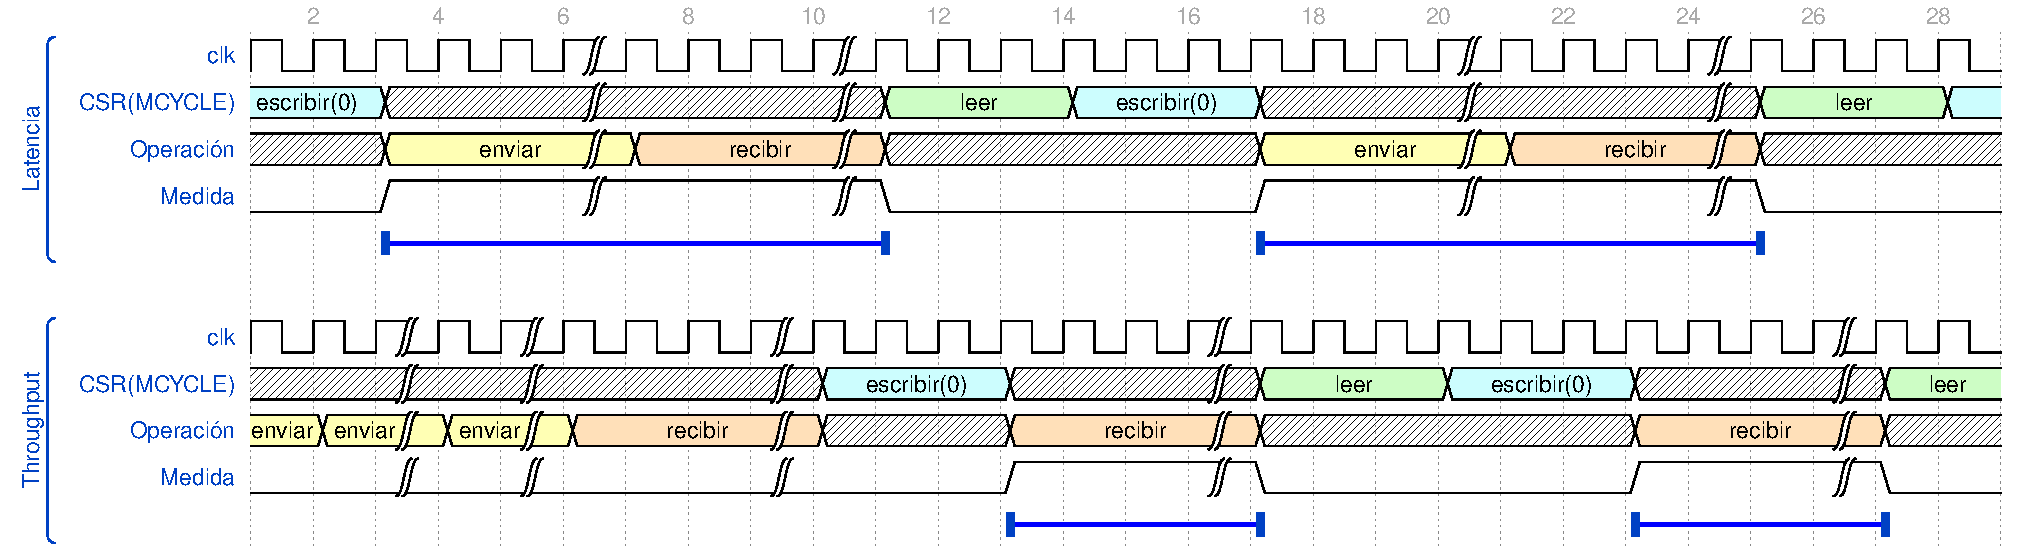
\includegraphics[width=14cm]{Figuras/wave_process.pdf}
    \caption{Aclaración gráfica de los dos tipos de ensayos: latencia y \textit{throughput}.}
    \label{fig:lat-thr}
\end{figure}

A este respecto, la parte de código destinada a simulación descrita en \ref{ap-cod:11}, \ref{ap-cod:12}, \ref{ap-cod:13} y \ref{ap-cod:12} para SLINK, XBUS, CFU Y CFS respectivamente, así como los respectivos \textit{test bench} de VUnit, se encargan de llevar a cabo estos ensayos.

Por último, cabe destacar que la evaluación mediante este método solo es posible para los ensayos del SoC completo, NEORV32 más multiplicador.
Para los ensayos mediante \textit{Verification Componets} se han empleado simulaciones de VUnit en conjunto con programas de Python encargados de gestionar los csv de salida producidos por la función \mintinline[breaklines]{vhdl}{info()} y así hacer los cálculos necesarios para obtener la latencia/\textit{throughput}.
En concreto, en el apéndice \ref{Codigo} se ejemplifica este proceso para la latencia de Mult-B acoplado mediante AXI-Stream.
Para ello se muestra el archivo que importa los VCs y extrae la información \ref{ap-cod:20}, el \textit{test bench} de VUnit \ref{ap-cod:21} y el \textit{script} de Python \ref{ap-cod:22} encargado de calcular a latencia.

\subsection{Ensayos de simulación}

%Tabla & Imagenes de integración continua
%Codigo de algun test bench de VUnit
%Se muestran los resultados en simulación obtenidos en integración continua en las imágenes.

Como se ha comentado en el apartado \ref{Workf}, la realización de las simulaciones está automatizada mediante la integración continua del repositorio.
En este sentido los 29 ensayos de simulación recogidos en la tabla \ref{tab:3} se han realizado con éxito y sus resultados se muestran de la figura \ref{fig:lat1} a la \ref{fig:thr9}.
Además, con objeto de facilitar la visualización estos resultados se resumen en la tabla \ref{tab:4}.

\begin{figure}[H]
    \centering
    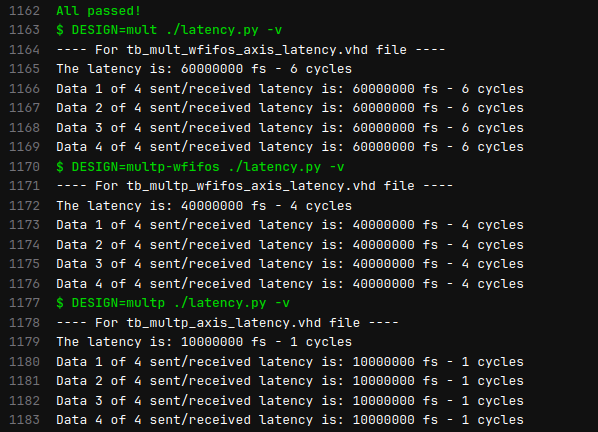
\includegraphics[width=14cm]{Figuras/result/lat1.png}
    \caption{Resultados del ensayo de latencia para Mult-B, Mult-BP y Mult-UBP acoplados mediante \textit{AXI-Stream Verification Componets}.}
    \label{fig:lat1}
\end{figure}

\begin{figure}[H]
    \centering
    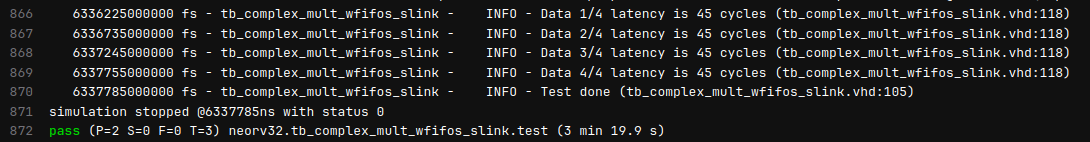
\includegraphics[width=14cm]{Figuras/result/lat2.png}
    \caption{Resultados del ensayo de latencia para NEORV32 + Mult-B, acoplado mediante SLINK.}
    \label{fig:lat2}
\end{figure}

\begin{figure}[H]
    \centering
    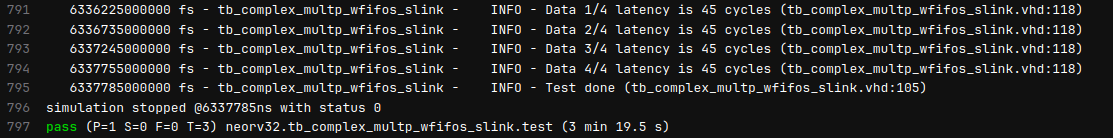
\includegraphics[width=14cm]{Figuras/result/lat3.png}
    \caption{Resultados del ensayo de latencia para NEORV32 + Mult-BP, acoplado mediante SLINK.}
    \label{fig:lat3}
\end{figure}

\begin{figure}[H]
    \centering
    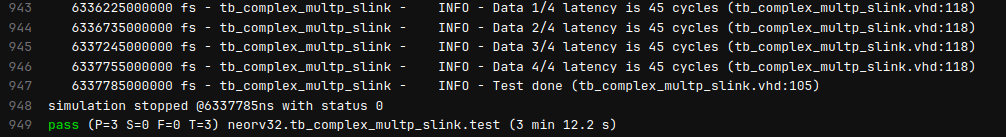
\includegraphics[width=14cm]{Figuras/result/lat4.png}
    \caption{Resultados del ensayo de latencia para NEORV32 + Mult-UBP, acoplado mediante SLINK.}
    \label{fig:lat4}
\end{figure}

\begin{figure}[H]
    \centering
    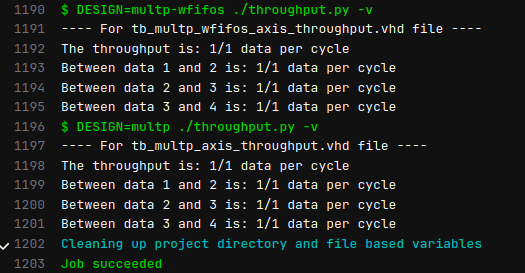
\includegraphics[width=14cm]{Figuras/result/thr1.png}
    \caption{Resultados del ensayo de \textit{throughput} para Mult-B, Mult-BP acoplados mediante \textit{AXI-Stream Verification Componets}.}
    \label{fig:thr1}
\end{figure}

\begin{figure}[H]
    \centering
    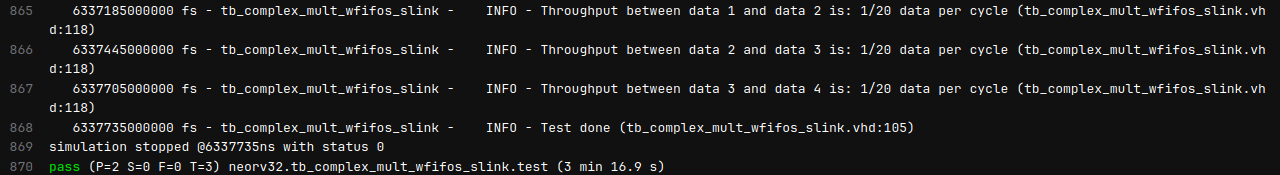
\includegraphics[width=14cm]{Figuras/result/thr2.png}
    \caption{Resultados del ensayo de \textit{throughput} para NEORV32 + Mult-B, acoplado mediante SLINK.}
    \label{fig:thr2}
\end{figure}

\begin{figure}[H]
    \centering
    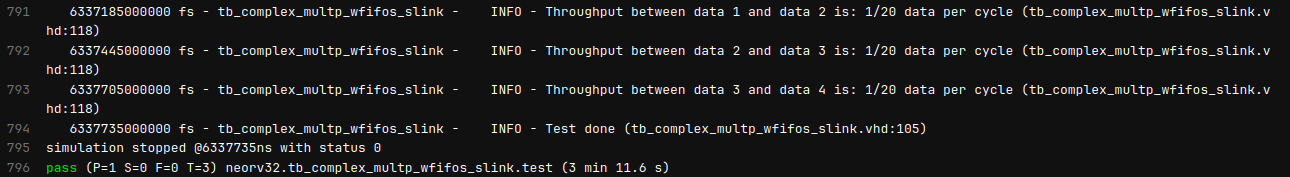
\includegraphics[width=14cm]{Figuras/result/thr3.png}
    \caption{Resultados del ensayo de \textit{throughput} para NEORV32 + Mult-BP, acoplado mediante SLINK.}
    \label{fig:thr3}
\end{figure}

\begin{figure}[H]
    \centering
    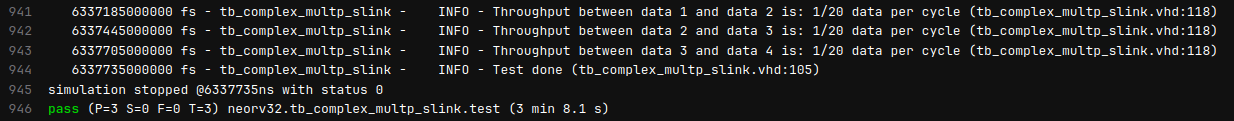
\includegraphics[width=14cm]{Figuras/result/thr4.png}
    \caption{Resultados del ensayo de \textit{throughput} para NEORV32 + Mult-UBP, acoplado mediante SLINK.}
    \label{fig:thr4}
\end{figure}

\begin{figure}[H]
    \centering
    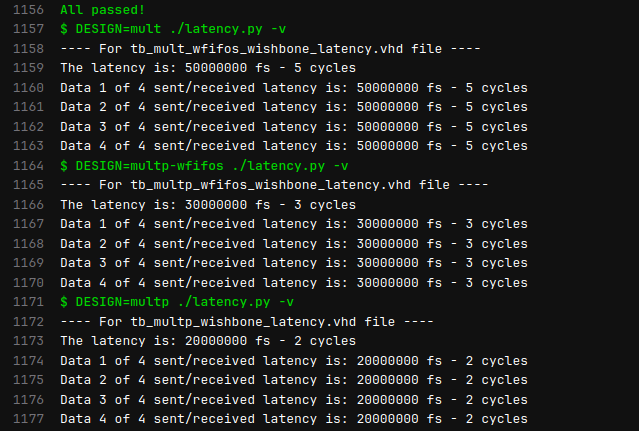
\includegraphics[width=14cm]{Figuras/result/lat5.png}
    \caption{Resultados del ensayo de latencia para Mult-B, Mult-BP y Mult-UBP acoplados mediante \textit{Wishbone Verification Componets}.}
    \label{fig:lat5}
\end{figure}

\begin{figure}[H]
    \centering
    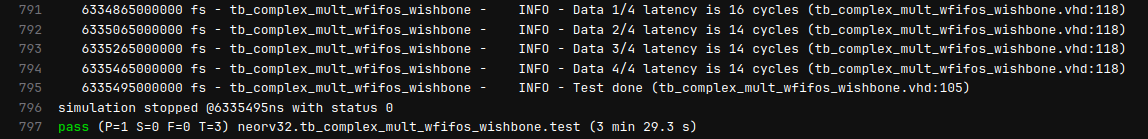
\includegraphics[width=14cm]{Figuras/result/lat6.png}
    \caption{Resultados del ensayo de latencia para NEORV32 + Mult-B, acoplado mediante XBUS.}
    \label{fig:lat6}
\end{figure}

\begin{figure}[H]
    \centering
    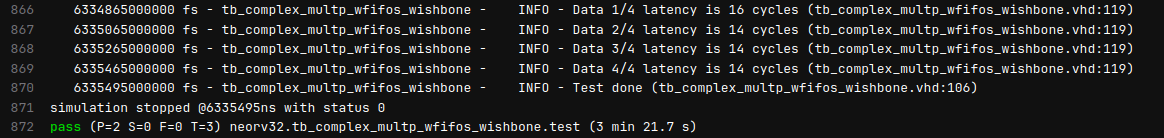
\includegraphics[width=14cm]{Figuras/result/lat7.png}
    \caption{Resultados del ensayo de latencia para NEORV32 + Mult-BP, acoplado mediante XBUS.}
    \label{fig:lat7}
\end{figure}

\begin{figure}[H]
    \centering
    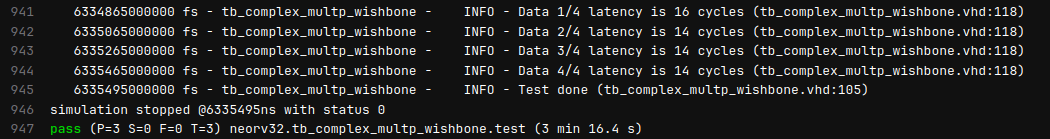
\includegraphics[width=14cm]{Figuras/result/lat8.png}
    \caption{Resultados del ensayo de latencia para NEORV32 + Mult-UBP, acoplado mediante XBUS.}
    \label{fig:lat8}
\end{figure}

\begin{figure}[H]
    \centering
    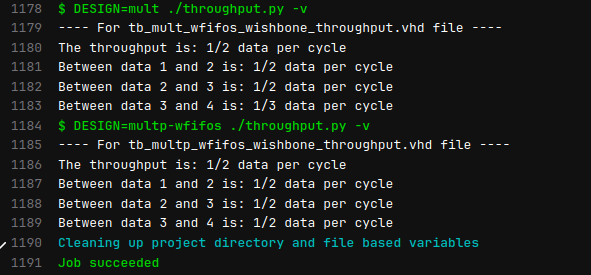
\includegraphics[width=14cm]{Figuras/result/thr5.png}
    \caption{Resultados del ensayo de \textit{throughput} para Mult-B, Mult-BP acoplados mediante \textit{Wishbone Verification Componets}.}
    \label{fig:thr5}
\end{figure}

\begin{figure}[H]
    \centering
    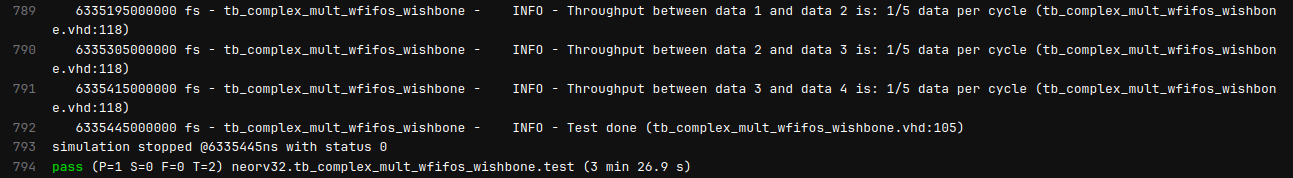
\includegraphics[width=14cm]{Figuras/result/thr6.png}
    \caption{Resultados del ensayo de \textit{throughput} para NEORV32 + Mult-B, acoplado mediante XBUS.}
    \label{fig:thr6}
\end{figure}

\begin{figure}[H]
    \centering
    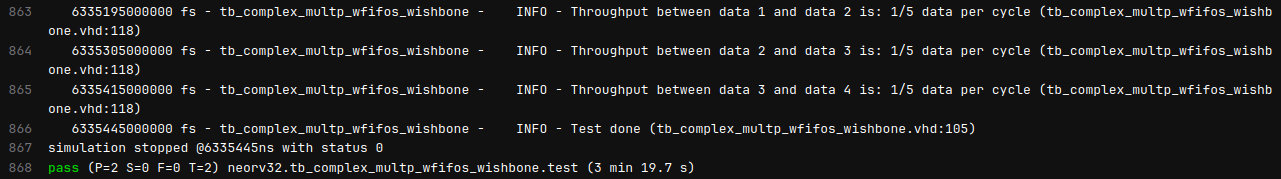
\includegraphics[width=14cm]{Figuras/result/thr7.png}
    \caption{Resultados del ensayo de \textit{throughput} para NEORV32 + Mult-BP, acoplado mediante XBUS.}
    \label{fig:thr7}
\end{figure}

\begin{figure}[H]
    \centering
    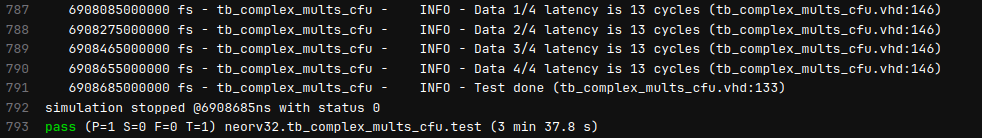
\includegraphics[width=14cm]{Figuras/result/lat9.png}
    \caption{Resultados del ensayo de latencia para NEORV32 + Mult-B, acoplado mediante CFU.}
    \label{fig:lat9}
\end{figure}

\begin{figure}[H]
    \centering
    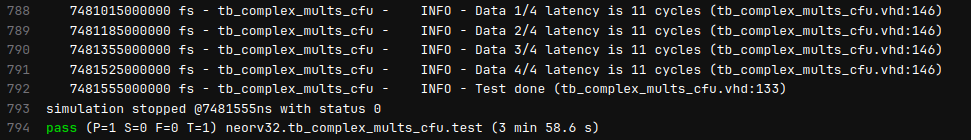
\includegraphics[width=14cm]{Figuras/result/lat10.png}
    \caption{Resultados del ensayo de latencia para NEORV32 + Mult-BP, acoplado mediante CFU.}
    \label{fig:lat10}
\end{figure}

\begin{figure}[H]
    \centering
    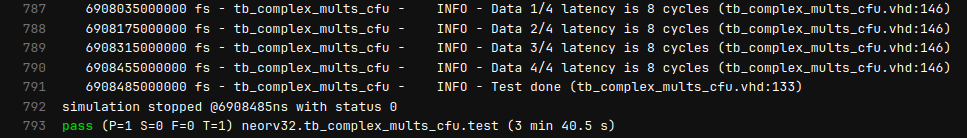
\includegraphics[width=14cm]{Figuras/result/lat11.png}
    \caption{Resultados del ensayo de latencia para NEORV32 + Mult-UBP, acoplado mediante CFU.}
    \label{fig:lat11}
\end{figure}

\begin{figure}[H]
    \centering
    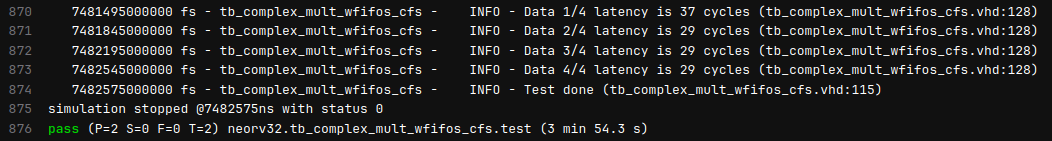
\includegraphics[width=14cm]{Figuras/result/lat12.png}
    \caption{Resultados del ensayo de latencia para NEORV32 + Mult-B, acoplado mediante CFS.}
    \label{fig:lat12}
\end{figure}

\begin{figure}[H]
    \centering
    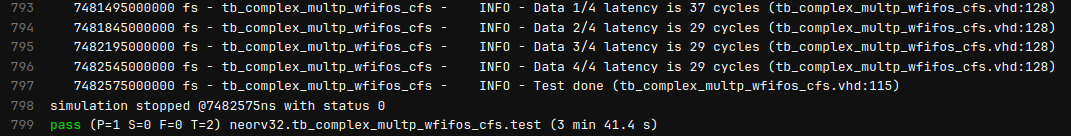
\includegraphics[width=14cm]{Figuras/result/lat13.png}
    \caption{Resultados del ensayo de latencia para NEORV32 + Mult-BP, acoplado mediante CFS.}
    \label{fig:lat13}
\end{figure}

\begin{figure}[H]
    \centering
    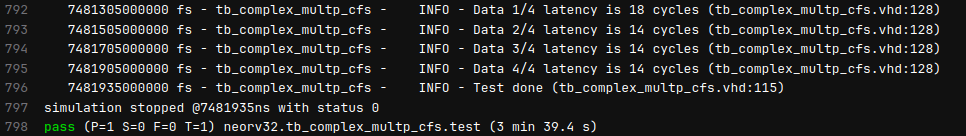
\includegraphics[width=14cm]{Figuras/result/lat14.png}
    \caption{Resultados del ensayo de latencia para NEORV32 + Mult-UBP, acoplado mediante CFS.}
    \label{fig:lat14}
\end{figure}

\begin{figure}[H]
    \centering
    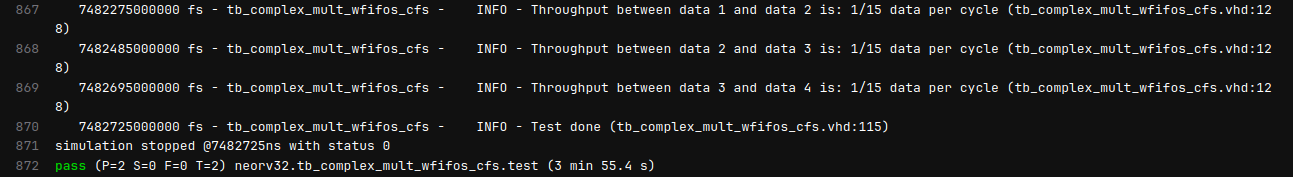
\includegraphics[width=14cm]{Figuras/result/thr8.png}
    \caption{Resultados del ensayo de \textit{throughput} para NEORV32 + Mult-B, acoplado mediante CFS.}
    \label{fig:thr8}
\end{figure}

\begin{figure}[H]
    \centering
    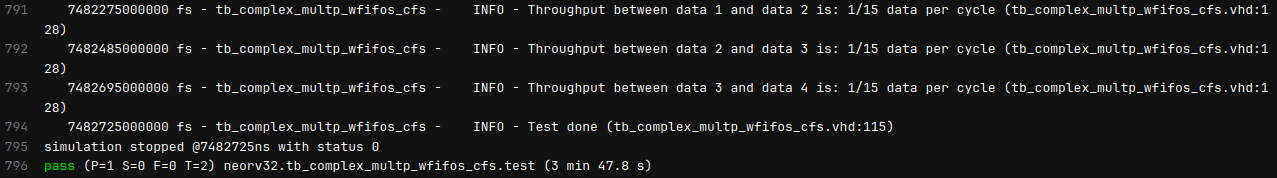
\includegraphics[width=14cm]{Figuras/result/thr9.png}
    \caption{Resultados del ensayo de \textit{throughput} para NEORV32 + Mult-BP, acoplado mediante CFS.}
    \label{fig:thr9}
\end{figure}

\begin{table}[h!]
\centering
\caption{Resultados de los ensayos de latencia y \textit{throughput}: VC, el multiplicador solo acoplado a \textit{Verification Components}; C, el SoC completo incluyendo el NEORV32, el multiplicador y la ejecución de software.}
\label{tab:4}
\begin{tabular}{|cc|cc|cc|c|c|}
\hline
\multicolumn{2}{|c|}{\multirow{2}{*}{\textbf{Mult}}}                                    & \multicolumn{2}{c|}{\textbf{SLINK}}           & \multicolumn{2}{c|}{\textbf{XBUS}}            & \textbf{CFU} & \textbf{CFS} \\ \cline{3-8} 
\multicolumn{2}{|c|}{}                                                                  & \multicolumn{1}{c|}{\textbf{VC}} & \textbf{C} & \multicolumn{1}{c|}{\textbf{VC}} & \textbf{C} & \textbf{C}   & \textbf{C}   \\ \hline
\multicolumn{1}{|c|}{\multirow{3}{*}{\textbf{Latencia}}}            & \textbf{Mult-B}   & \multicolumn{1}{c|}{6}           & 45         & \multicolumn{1}{c|}{5}           & 16         & 13           & 37           \\ \cline{2-8} 
\multicolumn{1}{|c|}{}                                              & \textbf{Mult-BP}  & \multicolumn{1}{c|}{4}           & 45         & \multicolumn{1}{c|}{3}           & 16         & 11           & 37           \\ \cline{2-8} 
\multicolumn{1}{|c|}{}                                              & \textbf{Mult-UBP} & \multicolumn{1}{c|}{1}           & 45         & \multicolumn{1}{c|}{2}           & 16         & 8            & 18           \\ \hline
\multicolumn{1}{|c|}{\multirow{3}{*}{\textit{\textbf{Throughput}}}} & \textbf{Mult-B}   & \multicolumn{1}{c|}{1/4}         & 1/20       & \multicolumn{1}{c|}{1/2}         & 1/5        & X            & 1/15         \\ \cline{2-8} 
\multicolumn{1}{|c|}{}                                              & \textbf{Mult-BP}  & \multicolumn{1}{c|}{1}           & 1/20       & \multicolumn{1}{c|}{1/2}         & 1/5        & X            & 1/15         \\ \cline{2-8} 
\multicolumn{1}{|c|}{}                                              & \textbf{Mult-UBP} & \multicolumn{1}{c|}{X}           & 1/20       & \multicolumn{1}{c|}{X}           & X          & X            & X            \\ \hline
\end{tabular}
\end{table}

\vspace{3cm}

Cabe destacar que por cada ensayo de simulación se ha producido un archivo .vcd que contiene las formas de onda producidas.
En este sentido, la integración continua se encarga de gestionar estos archivos y subirlos como artefactos.
En el apéndice \ref{wave}, se expone la forma de onda referente al ensayo de \textit{throughput} para NEORV32 + Mult-BP acoplado mediante XBUS \ref{wave:xbus} , así como la referente al ensayo de latencia para NEORV32 + Mult-B acoplado mediante CFU  \ref{wave:cfu}.

\subsection{Implementación en FPGA}

% captura cutecom de la implementación.

Todas las combinaciones del SoC, reflejadas en la figura \ref{fig:soc}, se han verificado tanto en la placa Arty A7 35T como en la 100T, lo que ha supuesto la generación duplicada de los \textit{bitstreams}.
Como se ha mencionado, el hecho de duplicar las placas permite asegurar una doble redundancia en la verificación.
Esta generación se ha realizado mediante las dos vías expuestas en la sección \ref{Workf}: herramientas FLOS y Vivado.
Con objeto de ilustrar cómo se aprecia la integración continua, en la imagen \ref{fig:impl-gh} se muestran los procesos para generar de forma automatizada los \textit{bitstreams} mediante herramientas FLOS en el repositorio de GitHub. 
En ella, se observa que se producen 18 artefactos, que contienen los \textit{bitstreams} y estarán almacenados en GitHub durante 90 días.
También se observa que la ejecución de los procesos es paralela, a diferencia de la relativa a Vivado en el CI de GitLab.
Debido a las características de gestión de procesos de Orion, el \textit{runner} asignado a Vivado solo permite la generación de \textit{bitstreams} de forma secuencial.
Este hecho aporta otro argumento que revalida la decisión de utilizar tanto herramientas FLOS como privativas.
Además, en el apendice \ref{Codigo} código \ref{ap-cod:23}, se muestra un ejemplo de un archivo bash realizado para generar automáticamente el \textit{bitstream} de la implementación CFU mediante herramientas FLOS.
En él, se observa un matiz destacable, al realizar la síntesis con yosys se añaden los argumentos  \mintinline[breaklines]{bash}{-nodsp} y \mintinline[breaklines]{bash}{-nolutram}.
Este hecho es debido a que la síntesis para la Arty mediante yosys no está del todo pulida, así como para Lattice sí, para Xilinix temas como la gestión de DSPs y de RAM distribuida todavía no están soportados.
Además, para obtener un correcto funcionamiento de los \textit{bitstreams} generados con herramientas FLOS, se ha tenido que rebajar la capacidad de la IMEM a:

\hspace{30mm} \mintinline[breaklines]{vhdl}{MEM_INT_IMEM_SIZE : natural := 6*1024}

\noindent Como se ha mencionado, además de la generación, el proceso de integración continua también automatiza la subida de los \textit{bitstreams} como artefactos.
En consecuencia, se han descargado y testeado todos ellos en ambas placas para comprobar su correcta operatividad.
En este sentido, se ha obteniendo un resultado satisfactorio.

\begin{figure}[H]
    \centering
    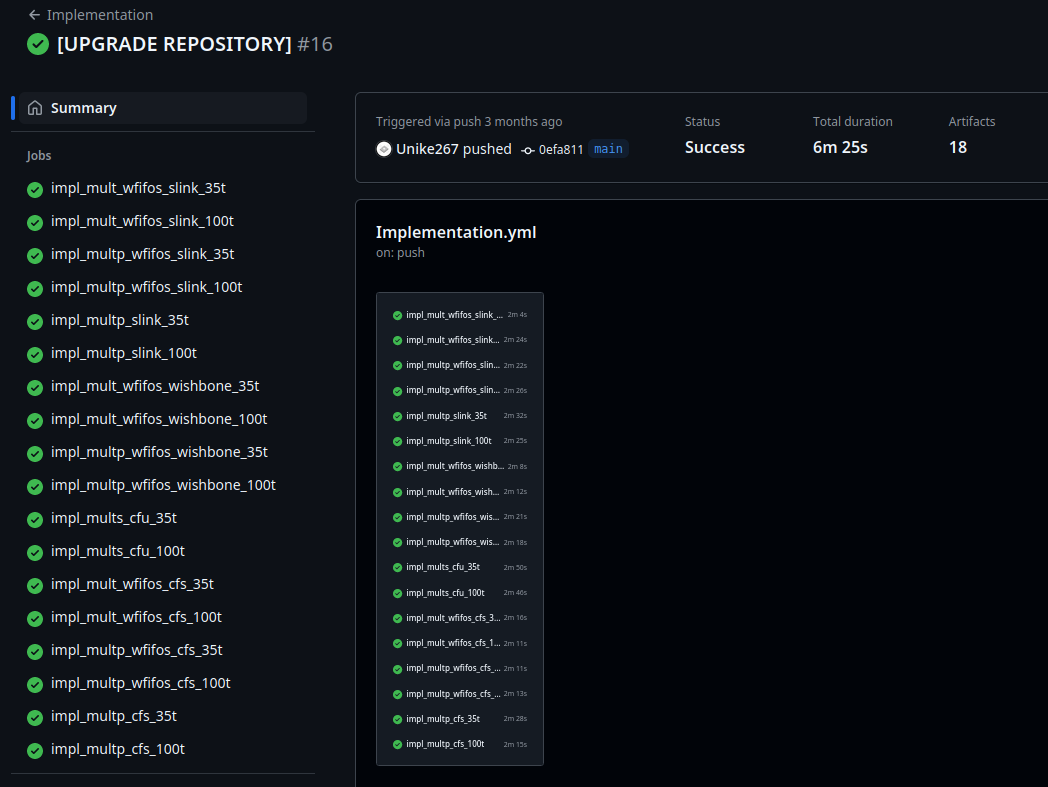
\includegraphics[width=14cm]{Figuras/impl-gh.png}
    \caption{Procesos de integración continua para generar los \textit{bitstreams} de los ensayos llevados a cabo mediante herramientas FLOS.}
    \label{fig:impl-gh}
\end{figure}

Los ensayos de implementación siguen un esquema similar a los ensayos de simulación.
No obstante, la finalidad no es realizar la caracterización del rendimiento, sino verificar la correcta operatividad.
En este sentido, todos los ensayos operan los mismos datos mediante el siguiente procedimiento.
Un programa de la IMEM, resultado de la compilación de la parte de código C destinada a implementación descrita en \ref{ap-cod:11}, \ref{ap-cod:12}, \ref{ap-cod:13} y \ref{ap-cod:12}, lanza 4 datos de entrada\footnote{Los datos de entrada son 1 x 1, 2 x 2, 4 x 4 y 8 x 8 (al igual que en simulación); por lo que se debe obtener en hexadecimal 0x1, 0x4, 0x10 (16) y 0x40 (64).} a los multiplicadores mediante cada método de acoplamiento, el acelerador los multiplica y los devuelve al NEORV32.
Además, las implementaciones muestran datos por UART, con objeto de visualizar en el ordenador la entrada y el resultado de cada operación, así como el tipo de ensayo.
De todos los ensayos en implementación realizados, se muestran cuatro con objeto de ejemplificar la correcta operatividad de los diseños.
Los resultados que se proceden a mostrar se han visualizado mediante la terminal CuteCom.
En concreto, la figura \ref{fig:impl1} refiere al multiplicador Mult-B acoplado al NEORV32 mediante SLINK, la figura \ref{fig:impl2} refiere al multiplicador Mult-BP acoplado mediante XBUS, la figura \ref{fig:impl3} refiere los tres multiplicadores acoplados mediante CFU y la figura \ref{fig:impl4} refiere al multiplicador Mult-UBP acoplado mediante CFS.

\begin{figure}[H]
    \centering
    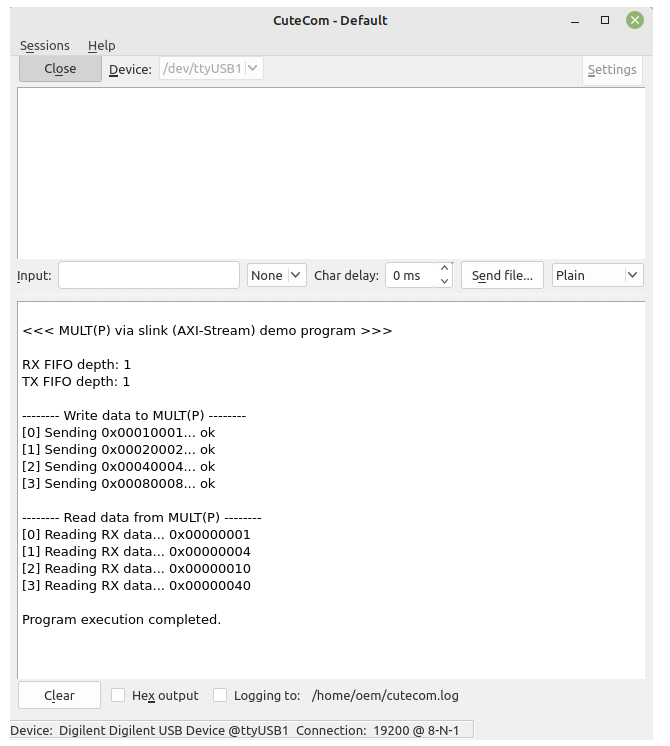
\includegraphics[width=14cm]{Figuras/impl1.png}
    \caption{Ensayo de implementación de Mult-B acoplado al NEORV32 mediante SLINK.}
    \label{fig:impl1}
\end{figure}

\begin{figure}[H]
    \centering
    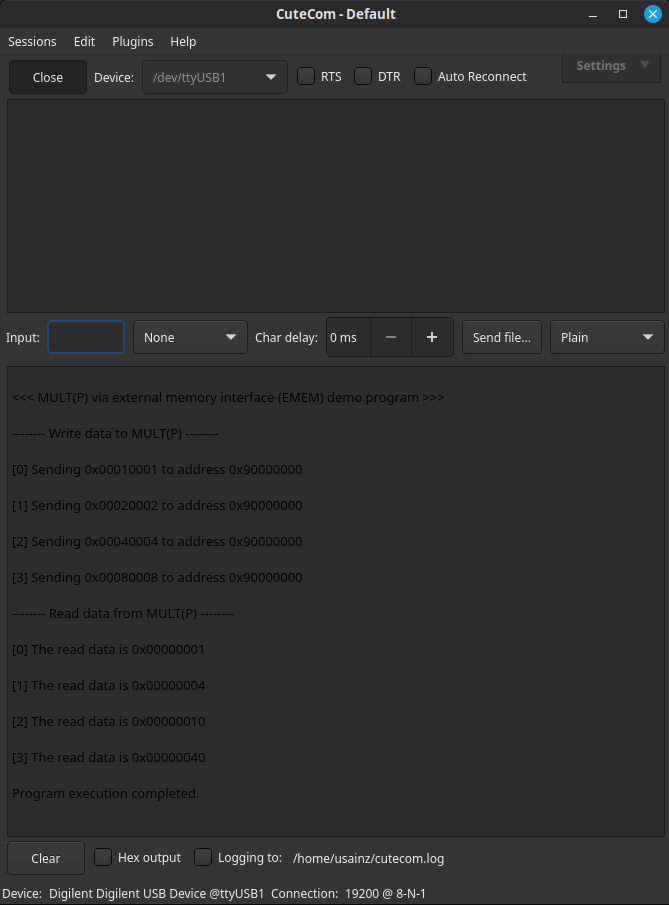
\includegraphics[width=14cm]{Figuras/impl2.png}
    \caption{Ensayo de implementación de Mult-BP acoplado al NEORV32 mediante XBUS.}
    \label{fig:impl2}
\end{figure}

\begin{figure}[H]
    \centering
    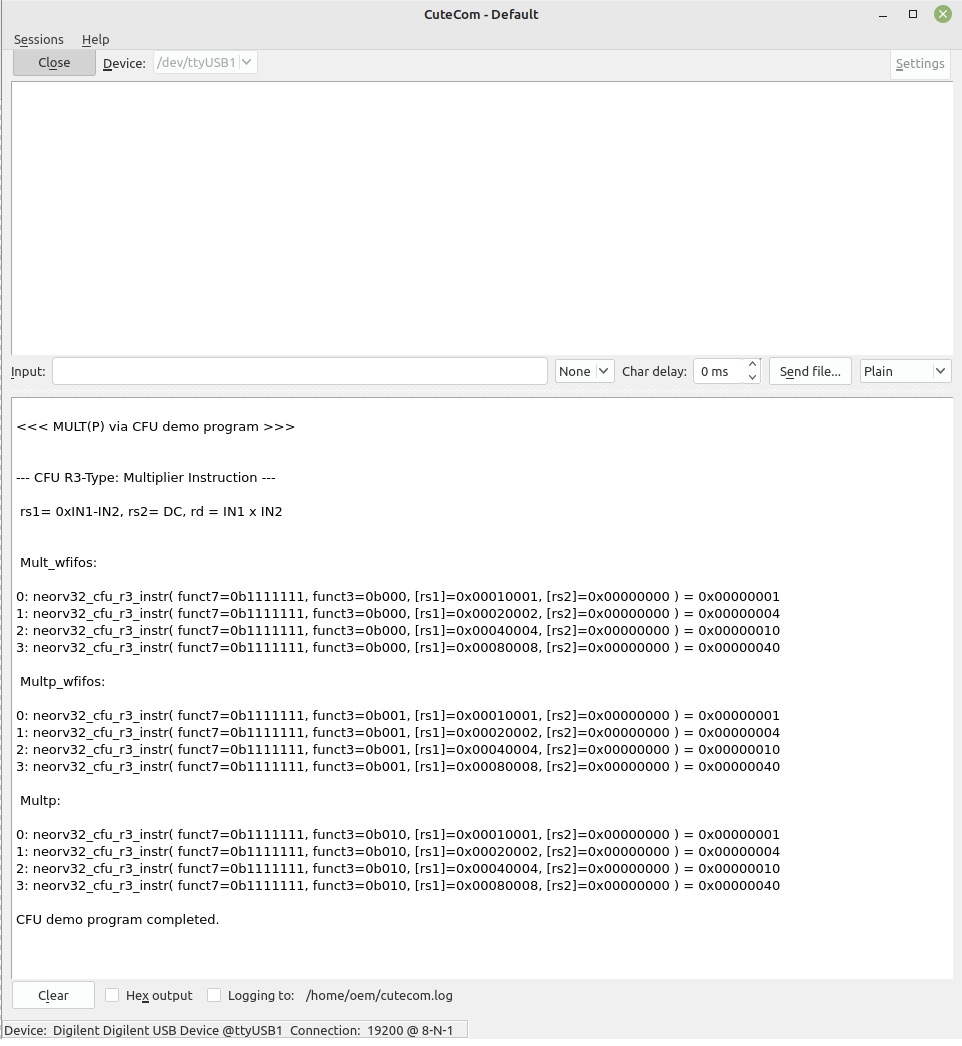
\includegraphics[width=14cm]{Figuras/impl3.png}
    \caption{Ensayo de implementación de Mult-B, Mult-BP y Mult-UBP acoplados al NEORV32 mediante CFU.}
    \label{fig:impl3}
\end{figure}

\begin{figure}[H]
    \centering
    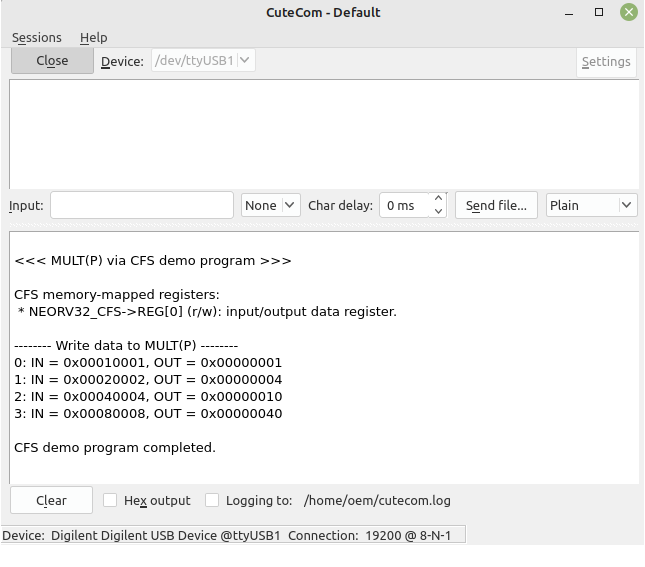
\includegraphics[width=14cm]{Figuras/impl4.png}
    \caption{Ensayo de implementación de Mult-UBP acoplado al NEORV32 mediante CFS.}
    \label{fig:impl4}
\end{figure}

\subsection{Análisis de los resultados}

\section{Integración de coprocesador para aplicaciones de IA}

\label{Integ}

Una vez generada la caracterización de todos los métodos de conexión, se cuenta con un criterio objetivo para escoger un modo de acoplamiento y conectar de forma óptima un coprocesador para acelerar aplicaciones de IA.
Como se ha mencionado, el coprocesador implementado únicamente se encarga de calcular la activación por medio de la función sigmoide.
%nexo
El procedimiento seguido para realizar la integración de este coprocesador se ha dividido en tres etapas. 
En la primera etapa, se realiza un ensayo de simulación del acelerador en solitario, además se acopla al NEORV32 mediante el método CFU con objeto de verificar en placa la correcta operatividad del mismo.
En la segunda etapa, se busca una manera de calcular la función de activación sigmoide haciendo uso de la unidad de coma flotante que ofrece el NEORV32.
En la tercera etapa, se realiza un ensayo comparativo, tanto en simulación como en implementación, para verificar las ventajas en términos de latencia de realizar el cálculo de la FA mediante un enfoque distribuido.

\subsection{Verificación de la operatividad del acelerador}

El acelerador ha sido proporcionado por el grupo de investigación.
Como se ha mencionado en \ref{cri}, este coprocesador acelera los cálculos mediante el método de interpolación recursiva centrada.
Cabe destacar que de las 7 funciones de activación disponibles solo se ha empleado la lógica de la función sigmoide.
Además, se han debido de hacer las debidas adaptaciones para conseguir la correcta operatividad del circuito en un entorno de VUnit.

El objetivo de la verificación es sencillo, se deben recrear los resultados obtenidos por Basterretxea para los 9 datos de entrada recogidos en la tabla \ref{tab:5}.
Para ello se comienza con una simulación del coprocesador en solitario en el entorno de VUnit.
Después, se acopla al NEORV32 mediante CFU y se realiza una implementación en placa.
En este sentido, el NEORV32 se encargará de enviar los 9 datos de entrada al coprocesador, asimismo este calculará y devolverá el resultado de la FA de vuelta al microcontrolador.
Tanto el ensayo en simulación del coprocesador en solitario como la generación del \textit{bitstream} del ensayo en implementación del coprocesador acoplado al NEORV32 mediante CFU, se realizan mediante tareas automatizadas en la integración continua del repositorio de GitLab.
Estos ensayos no se encuentran disponibles en el repositorio propio de GitHub.

\begin{table}[h!]
\centering
\caption{Resultados de la función sigmoide a verificar.}
\label{tab:5}
\begin{tabular}{|c|ccc|}
\hline
\multirow{3}{*}{\textbf{Dato de entrada}} & \multicolumn{3}{c|}{\textbf{Resultado de la función sigmoide}}                                           \\ \cline{2-4} 
                                          & \multicolumn{2}{c|}{\textbf{Matlab}}                                                & \textbf{Modelsim}  \\ \cline{2-4} 
                                          & \multicolumn{1}{c|}{\textbf{Coma fija}} & \multicolumn{1}{c|}{\textbf{Hexadecimal}} & \textbf{Coma fija} \\ \hline
-10                                       & \multicolumn{1}{c|}{0}                  & \multicolumn{1}{c|}{0000}                 & 0                  \\ \hline
-7,5                                      & \multicolumn{1}{c|}{0,0078125}          & \multicolumn{1}{c|}{0002}                 & 0,0078125          \\ \hline
-5                                        & \multicolumn{1}{c|}{0,15625}            & \multicolumn{1}{c|}{0028}                 & 0,15625            \\ \hline
-2,5                                      & \multicolumn{1}{c|}{0,484375}           & \multicolumn{1}{c|}{007C}                 & 0,484375           \\ \hline
0                                         & \multicolumn{1}{c|}{1}                  & \multicolumn{1}{c|}{0100}                 & 1                  \\ \hline
2,5                                       & \multicolumn{1}{c|}{1,515625}           & \multicolumn{1}{c|}{0184}                 & 1,515625           \\ \hline
5                                         & \multicolumn{1}{c|}{1,84375}            & \multicolumn{1}{c|}{01D8}                 & 1,84375            \\ \hline
7,5                                       & \multicolumn{1}{c|}{1,9921875}          & \multicolumn{1}{c|}{01FE}                 & 1,9921875          \\ \hline
10                                        & \multicolumn{1}{c|}{2}                  & \multicolumn{1}{c|}{0200}                 & 2                  \\ \hline
\end{tabular}
\end{table}

Los resultados obtenidos en simulación del coprocesador en solitario se muestran en la figura \ref{fig:sim_alone}, así como los obtenidos en implementación para el coprocesador acoplado al NEORV32 vía CFU se muestran en la figura \ref{fig:impl_complex}.
Asimismo, el código que describe el acelerador utilizado se encuentra en el apéndice \ref{Codigo} código \ref{ap-cod:24}, así como la integración en CFU se muestra en el código \ref{ap-cod:25}.
Además, se aclara gráficamente la integración del acelerador mediante CFU en el plano \ref{}. 
%hacer plano con latex
Por último, se muestra la forma de onda resultante del cálculo de dos sigmoides por el acelerador CRI mediante CFU en el apéndice, \ref{wave} forma de onda \ref{wave:sig}. 
En esta forma de onda se observa algo interesante, las señales de la CFU varían con respecto a la forma de onda \ref{wave:cfu} (implementación del multiplicador).
Esto es debido a que en el transcurso de la elaboración de esta investigación la integración mediante CFU cambió ligeramente, como se ha mencionado en el apartado \ref{neorv32}.
%hacer forma de onda
Al igual que para el caso del multiplicador, se emplea una instrucción personalizada \textit{R3-Type} de la extensión Zxcfu.
Se emplea el registro fuente \textit{rs1} para la entrada del acelerador.
Ya que los datos a verificar se generaron con una longitud de palabra WL = 16 bits, se ha querido preservar el acelerador a este tamaño de entrada/salida para todos los ensayos realizados en este capítulo.
En este sentido, en el código \ref{ap-cod:25} se observa como se ha gestionado este longitud con el tamaño de los registros \textit{rs1} y \textit{rd} de 32 bits. 
El registro fuente \textit{rs2} no se utiliza y el resultado del cálculo de la función sigmoide se guarda en el registro de destino \textit{rd}.
Para especificar la función se ha empleado el campo \textit{funct3}, asociando el coprocesador sigmoide a \mintinline[breaklines]{c}{funct3=000}.

%Añadir la flexibilidad de cli, se puede ajustar a distintos q + x ciclos

\begin{figure}[H]
    \centering
    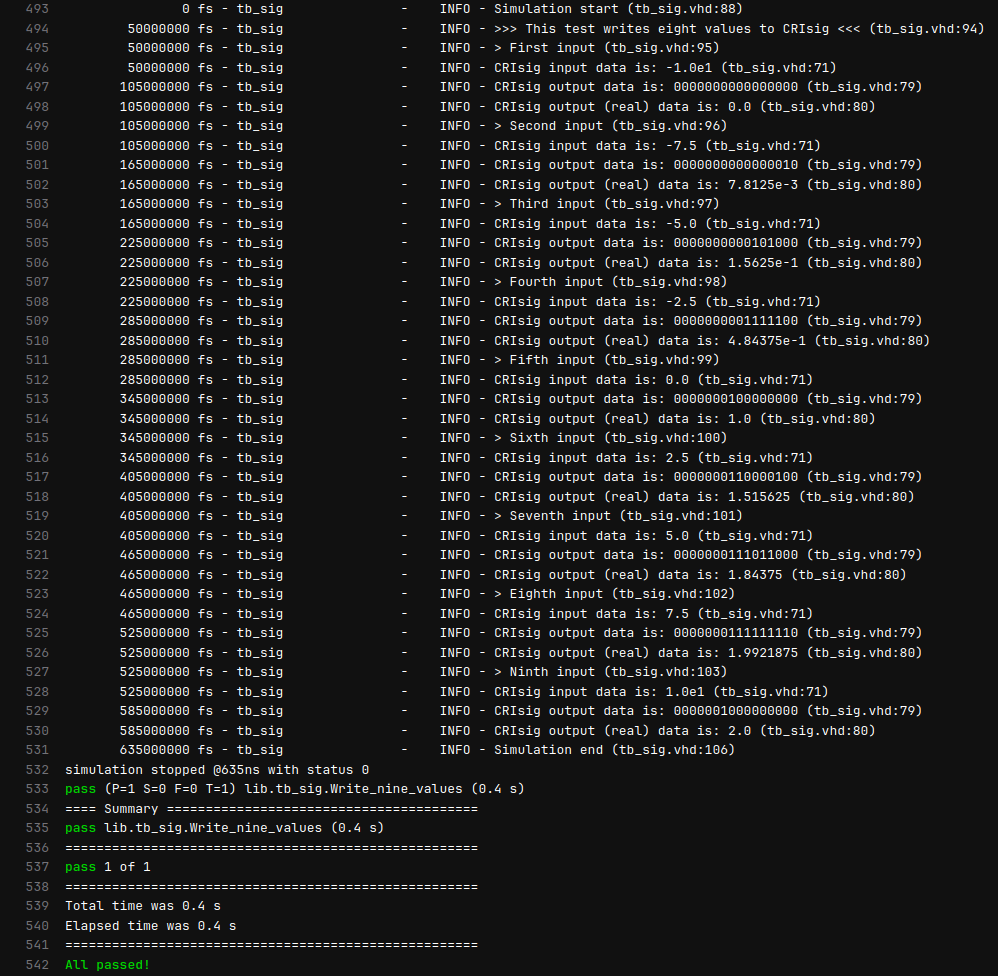
\includegraphics[width=14cm]{Figuras/sim_sig_alone.png}
    \caption{Verificación en simulación de la correcta operatividad del acelerador sigmoide en un entorno de VUnit.}
    \label{fig:sim_alone}
\end{figure}

\begin{figure}[H]
    \centering
    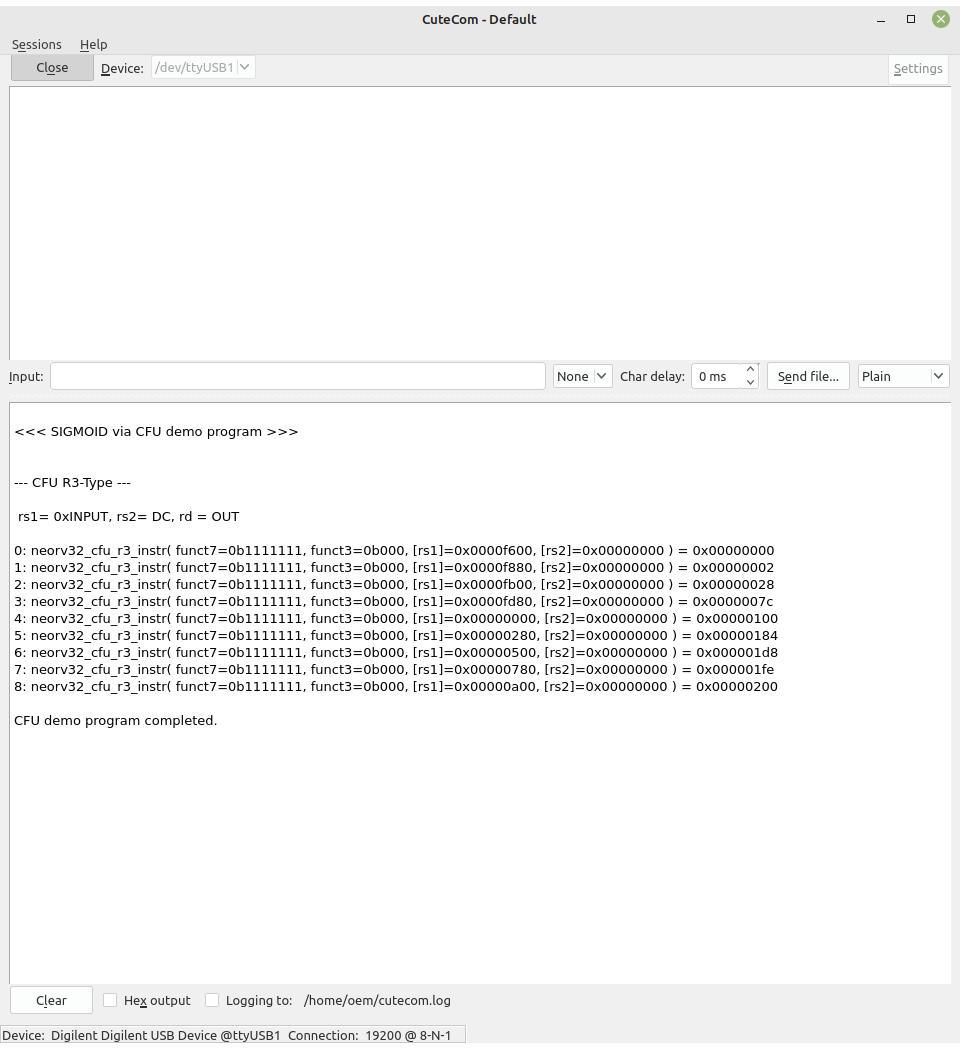
\includegraphics[width=14cm]{Figuras/sig_cfu.png}
    \caption{Verificación en implementación de la correcta operatividad del acelerador sigmoide acoplado al NEORV32 mediante CFU.}
    \label{fig:impl_complex}
\end{figure}

Como se puede apreciar en las imágenes los resultados en ambos casos han sido los esperados, cumpliendo de forma óptima la primera etapa de verificación.

\subsection{Realización del cálculo de la FA mediante la FPU}

\label{fpu-fa}

La tarea de calcular la función de activación sigmoide mediante los recursos por defecto del NEORV32, se ha decidido implementar mediante la Unidad de Coma Flotante (FPU).
%si da tiempo hacer ensayo de mult float sin FPU
Es decir, al contrario que el acelerador que se usa coma fija, para el enfoque realizado sin coprocesador se emplean datos en coma flotante.
Normalmente, cuando una red se calcula por software, es decir, sin externalizar los cálculos a coprocesadores embebidos, los datos que se suelen usar son de este tipo, por lo que se ha visto adecuado emular este hecho.
En concreto, las instrucciones relativas al manejo de la Unidad de Coma Flotante se encuentran en la extensión Zfinx.
En este sentido surge un pequeño inconveniente.
Debido a que la implementación hardware actual de la extensión en el NEORV32 es limitada, esta \href{https://stnolting.github.io/neorv32/#_zfinx_isa_extension}{no soporta operaciones de división}.
A priori, esto puede resultar un problema.
Ya que la función sigmoide es una fracción \eqref{ec:2}, resolverla sin emplear operaciones de división puede resultar engorroso.
Es por ello que se ha buscado una alternativa de cálculo.
En primer lugar, se ha de tener en cuenta que las operaciones de suma y de multiplicación sí que están soportadas mediante las funciones \mintinline[bgcolor=pink,breaklines]{c}{riscv_intrinsic_fadds()} y \mintinline[bgcolor=pink,breaklines]{c}{riscv_intrinsic_fmuls()} respectivamente.
Este hecho nos abre una ventana de posibilidad y nos permite implementar una aproximación polinomial a la función sigmoide.
Para ello se ha realizado un programa en python descrito en el código \ref{ap-cod:26}.
Este programa hace uso de la librería numpy y su funcionamiento es la siguiente: se describe la función a aproximar, en este caso \eqref{ec:3} (sigmoide ajustada a saturación = 2 y pendiente = 0,5), se calculan los coeficientes para tres grados distintos de polinomios y se realiza una gráfica comparativa.
Cabe destacar que el rango de aproximación definido está condicionado por los valores a testear, es decir, entre -10 y 10.
Se decide realizar polinomios de grado 3\eqref{ec:4}, 5\eqref{ec:5} y 7\eqref{ec:6} con objeto de testear varías implementaciones y no comprometer ni el tiempo de ejecución ni la precisión, obteniendo varios ejemplos a comparar con el coprocesador. 

\begin{equation}\label{ec:3}
f(x)= 2 \times \frac{1}{1 + e^{-0,5x}}\tag{***}
\end{equation}

Los polinomios de aproximación a la función sigmoide obtenidos son los siguientes:

\begin{equation}\label{ec:4}
f(x)= 1 + 0.19744040439x -0.00109773200x^3\tag{****}
\end{equation}


\begin{equation}\label{ec:5}
f(x)= 1 +  0.22878851178x - 0.00253272801x^3 + 0.00001266682x^5\tag{*****}
\end{equation}

\begin{equation}\label{ec:6}
f(x)= 1 + 0.24190955524x - 0.00369209483x^3 + + 0.00003770457x^5 - 0.00000015213x^7 \tag{******}
\end{equation}

En la figura \ref{fig:comp}, se observa el resultado de las aproximaciones polinómicas propuestas para aproximar la función sigmoide en el rango indicado.
En este sentido, en el código \ref{ap-cod:27} se puede observar como se implementan estas funciones en C.
Además, cabe destacar que el NEORV32 no soporta la impresión de flotantes por UART, por lo que se ha tenido que adaptar el resultado a dos enteros que representen la parte entera y la parte decimal.
Para este propósito, entre otras cosas, se ha utilizado la función \mintinline[bgcolor=pink,breaklines]{c}{riscv_intrinsic_flts()} para realizar la comparación \say{menor que} de un flotante con cero y evaluar su signo.
Para emplear las funciones de la extensión Zfinx, esta se debe activar en el TOP del diseño.

\hspace{32mm} \mintinline[breaklines]{vhdl}{CPU_EXTENSION_RISCV_Zfinx => true} 

\begin{figure}[H]
    \hspace*{-38mm}
    \centering
    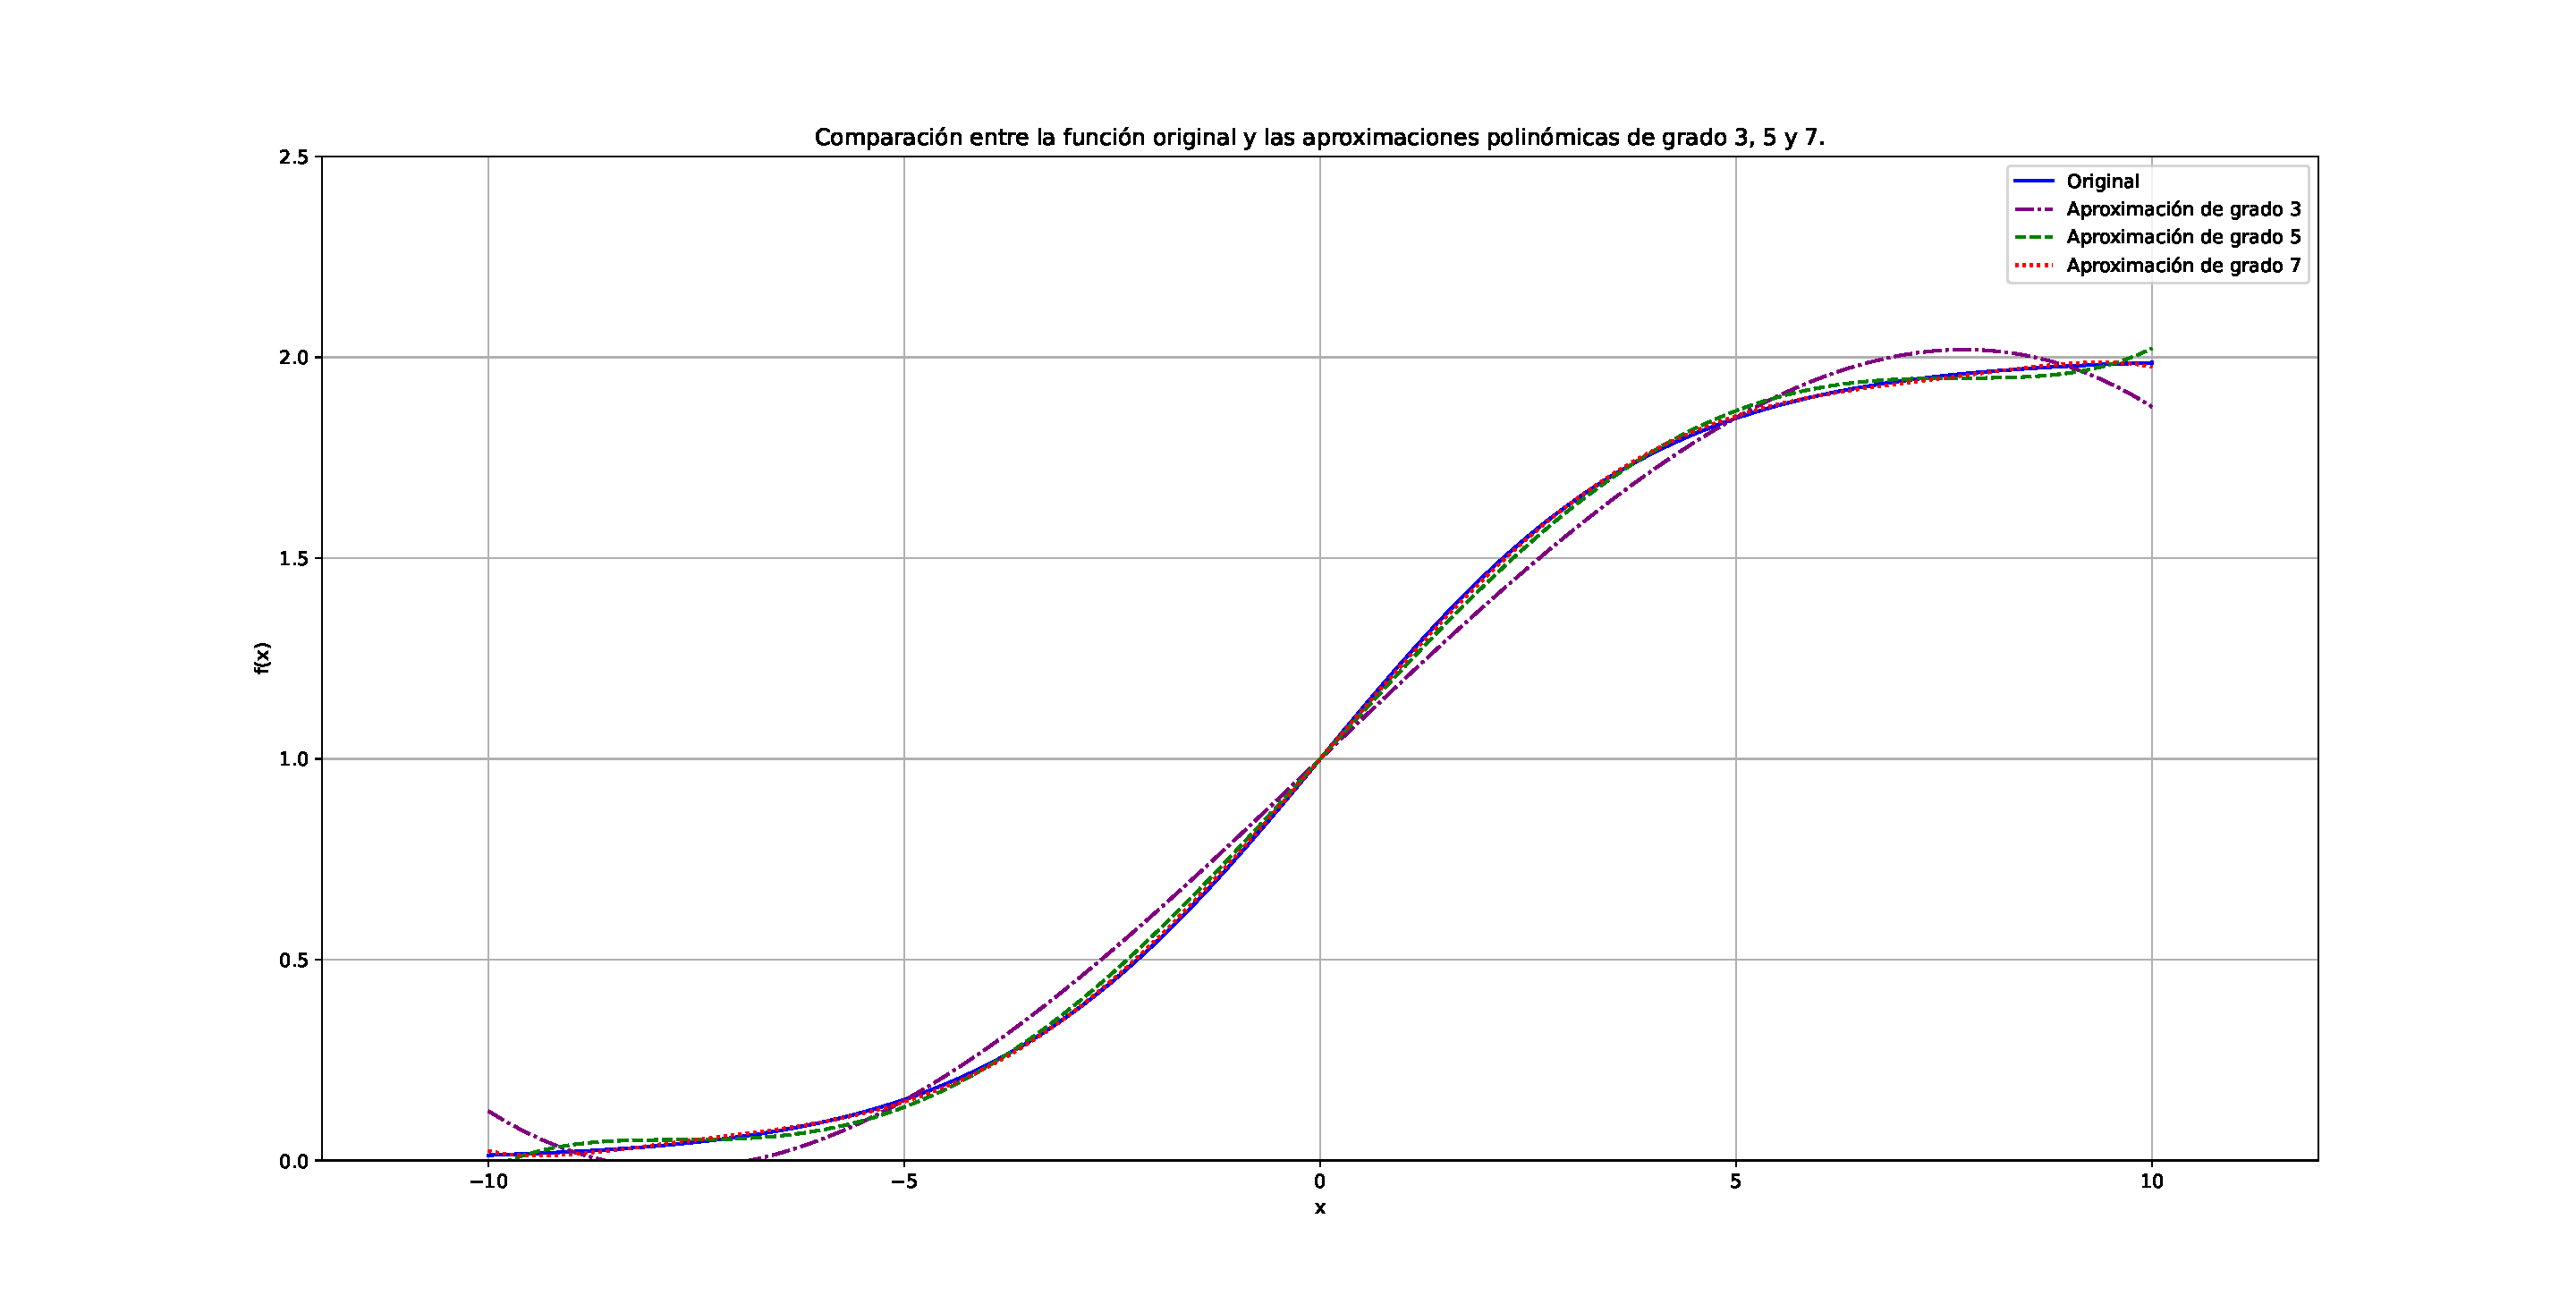
\includegraphics[width=22cm]{Figuras/Comp_aprox.pdf}
    \caption{Comparación entre la función original y las aproximaciones polinómicas de grado 3, 5 y 7.}
    \label{fig:comp}
\end{figure}

Cabe destacar un hecho relevante, como se ha mencionado las aproximaciones polinómicas están calculadas en función del rango propuesto.
Es decir, su uso no se puede generalizar para todos los valores de entrada de la recta real.
Esto se debe a que, para valores fuera del rango indicado, el polinomio se puede inestabilizar y desviar por completo de la aproximación a la función sigmoide.
Además, para las aproximaciones de grado 3 y 5, las colas en los extremos no son aceptables.
En consecuencia, para una aplicación real, el inicio y el final de estas aproximaciones se deben saturar a 0 y a 2, respectivamente.

\subsection{Comparación de enfoques}

La comparación de ambos enfoques se ha llevado a cabo mediante una simulación de VUnit  y una implementación en placa.
Tanto la simulación, como la generación del \textit{bitstream} del ensayo en placa, se han automatizo en tareas de integración continua del repositorio de GitLab.
Estos ensayos no se encuentran disponibles en el repositorio propio de GitHub.

\subsubsection{Simulación}

El ensayo de simulación consiste en lanzar un mismo paquete de 9 datos 4 veces, un vez por cada implementación sigmoide a testear y medir los ciclos que tarda cada una de ellas en calcular el resultado para cada dato de entrada.
En este sentido, se ha acoplado mediante CFU el coprocesador CRI al NEORV32 con su FPU activada, con la cual se calculan las otras tres implementaciones.
El orden seguido es el siguiente, en primer lugar se lanza el paquete al acelerador CRI, en segundo lugar a la aproximación polinómica de grado 7, en tercer lugar a la aproximación polinómica de grado 5 y por último a la aproximación polinómica de grado 3, 36 datos en total.
Para realizar las medidas de latencia, se ha utilizado la metodología expuesta en el apartado \ref{met}.
El código empleado en esta simulación se encuentra en la parte de código destinada a simulación del programa \ref{ap-cod:27}.
Los resultados obtenidos se muestran en la figura \ref{fig:sim_comp}

\begin{figure}[H]
    \centering
    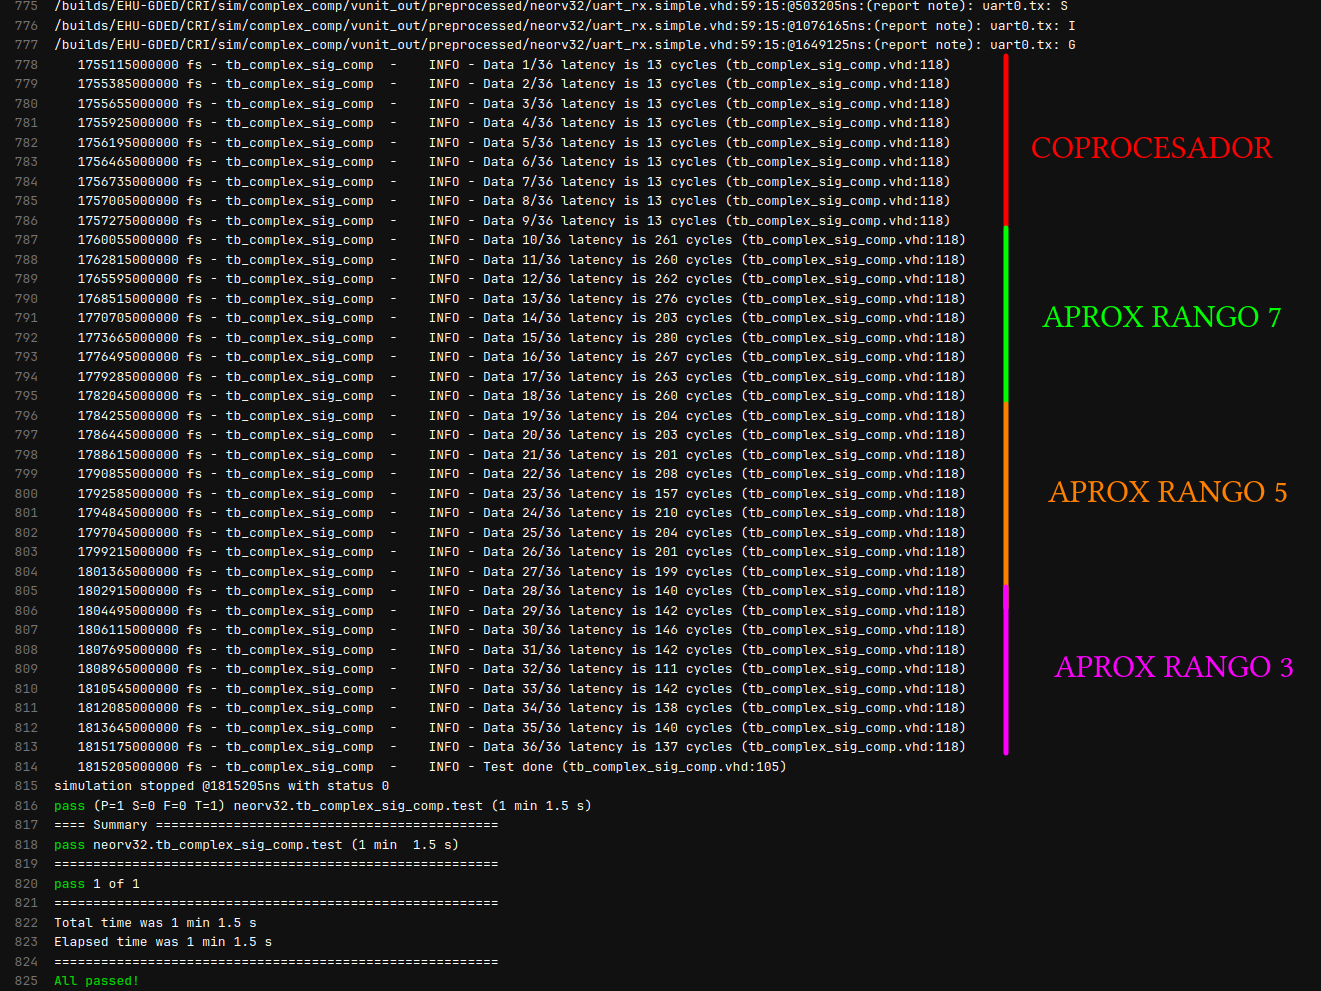
\includegraphics[width=14cm]{Figuras/SIM_RES_CI.png}
    \caption{Resultados de simulación en ciclos de latencia necesarios para calcular la función sigmoide para cada dato de entrada.}
    \label{fig:sim_comp}
\end{figure}

\subsubsection{Implementación}

El ensayo en placa ha consistido en dos partes contenidas en un mismo programa, ver la parte de código destinada a implementación en \ref{ap-cod:27}.
Por un lado, se ha computado el resultado de la función sigmoide con los dos enfoques, el distribuido mediante el coprocesador acoplado al NEORV32 y el monolítico a través de las tres aproximaciones mediante la FPU.
Para ello, se han utilizado los mismo 9 datos de entrada que en simulación.
Por otro lado, se ha repetido cada uno de estos cómputos y mediante el uso del CSR(mcycle) se ha calculado la latencia que tarda cada uno de los enfoques en calcular un paquete completo de datos, dando un punto de vista más global.
La figura \ref{fig:impl_comp} muestra el resultado del ensayo transmitido por UART y visualizado mediante la terminal CuteCom.

\begin{figure}[H]
    \centering
    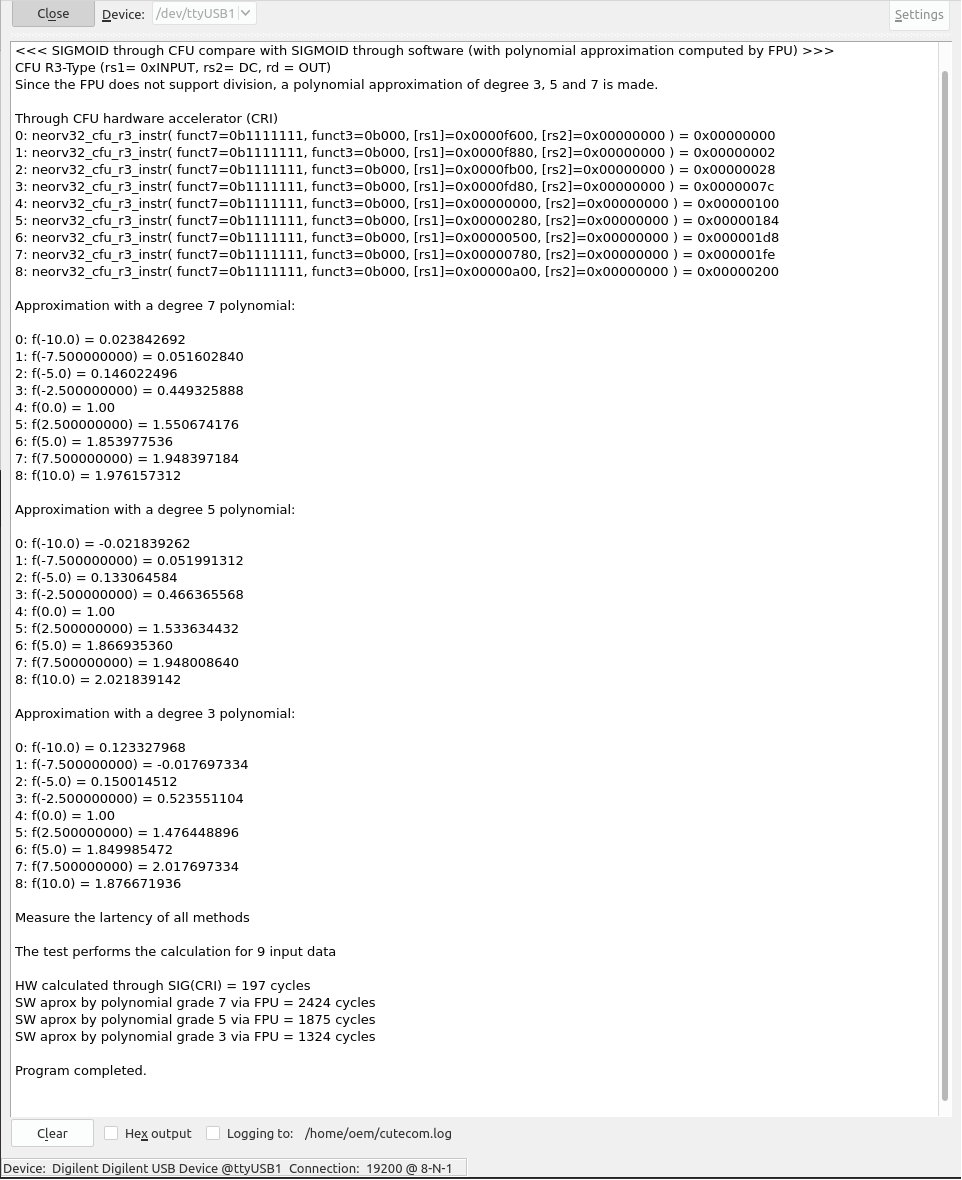
\includegraphics[width=14cm]{Figuras/RES_impl_comp.png}
    \caption{Resultado del ensayo comparativo en placa.}
    \label{fig:impl_comp}
\end{figure}

\subsubsection{Resultados}

Se procede a agrupar los resultados obtenidos en dos tablas.
Una referente al resultado del cálculo de la función sigmoide \ref{tab:6} y otra a la latencia relativa a cada implementación \ref{tab:7}.

Respecto a los resultados de la sigmoide, se observa que para los valores cercanos a los límites del rango relativos a las aproximaciones de grado bajo es necesario realizar una saturación, como ya se ha destacado en la subsección \ref{fpu-fa}.
No obstante, la aproximación de grado más alto se ajusta con relativa eficacia a los valores esperados.
Respecto a la latencia, cabe destacar que la mínima para los casos de las aproximaciones mediante FPU coincide siempre con el 5º dato, el cual es f(0) = 1.
De este hecho se deduce que se requiere poca carga computacional para calcular esa salida, es por ello que baja tanto su resultado.
Si se observan el resto de casos, figura \ref{fig:sim_comp}, la desviación no es tan notable.
Respecto a los resultados del paquete de datos se aprecia que no se ajusta de forma directa al total de ciclos entre 9.
Esto es debido a que en el ensayo de simulación se mide rigurosamente cada ejecución de dato aislada, mientras que la implementación en placa mide, aparte de la ejecución per se, las instrucciones relativas al bucle for que corre la secuencia de introducción del paquete, lo que añade ciclos extra a la computación, ver \ref{ap-cod:27}.
Es por ello que se ha mencionado que el ensayo en placa da un punto de vista más global.
Debido a que en la práctica no solo se ejecutan los ciclos relativos a las instrucciones propias, es de interés medir la parte del código añadido que compone la aplicación.
Respecto al ahorro computacional en ciclos de latencia obtenidos mediante el acelerador CRI, se afirma que en el caso más ajustado se ahorran 111 - 13 = 98 ciclos por dato, lo cual es una aceleración de 8,53:1 y en el caso más holgado se ahorran 280 - 13 = 267 ciclos por dato, lo cual es una aceleración de 21,53:1.
Si se realiza la media de las tres medias y se compara se obtiene un ahorro de 198,3 - 13 = 185,3 ciclos por dato, lo cual es una aceleración de 15,25:1.
Estos hechos corroboran el beneficio de emplear este tipo de enfoque distribuido y afianzan el argumento de externalizar los cálculos relativos a las redes neuronales a coprocesadores embebidos con la finalidad de llevar a cabo una gestión computacional eficaz y simplificada de IA en el borde.


%tabla de resultados

\begin{table}[H]
\centering
\caption{Resultados de la función sigmoide obtenidos mediante los cuatro casos ensayados (implementación).}
\label{tab:6}
\begin{tabular}{|c|cc|ccc|}
\hline
\multirow{3}{*}{\textbf{Entrada}} & \multicolumn{2}{c|}{\multirow{2}{*}{\textbf{\begin{tabular}[c]{@{}c@{}}Coprocesador\\ CRI\end{tabular}}}} & \multicolumn{3}{c|}{\textbf{Aproximación mediante FPU}}                                          \\ \cline{4-6} 
                                  & \multicolumn{2}{c|}{}                                                                                     & \multicolumn{1}{c|}{\textbf{Grado 7}} & \multicolumn{1}{c|}{\textbf{Grado 5}} & \textbf{Grado 3} \\ \cline{2-6} 
                                  & \multicolumn{1}{c|}{\textbf{Coma fija}}                       & \textbf{Hexadecimal}                      & \multicolumn{3}{c|}{\textbf{Coma flotante}}                                                      \\ \hline
-10                               & \multicolumn{1}{c|}{0}                                        & 0000                                      & \multicolumn{1}{c|}{0,023842692}      & \multicolumn{1}{c|}{-0,021839262}     & 0,123327968      \\ \hline
-7,5                              & \multicolumn{1}{c|}{0,0078125}                                & 0002                                      & \multicolumn{1}{c|}{0,051602840}      & \multicolumn{1}{c|}{0,051991312}      & -0,017697334     \\ \hline
-5                                & \multicolumn{1}{c|}{0,15625}                                  & 0028                                      & \multicolumn{1}{c|}{0,146022496}      & \multicolumn{1}{c|}{0,133064584}      & 0,150014512      \\ \hline
-2,5                              & \multicolumn{1}{c|}{0,484375}                                 & 007C                                      & \multicolumn{1}{c|}{0,449325888}      & \multicolumn{1}{c|}{0,466365568}      & 0,523551104      \\ \hline
0                                 & \multicolumn{1}{c|}{1}                                        & 0100                                      & \multicolumn{1}{c|}{1,00}             & \multicolumn{1}{c|}{1,00}             & 1,00             \\ \hline
2,5                               & \multicolumn{1}{c|}{1,515625}                                 & 0184                                      & \multicolumn{1}{c|}{1,550674176}      & \multicolumn{1}{c|}{1,533634432}      & 1,476448896      \\ \hline
5                                 & \multicolumn{1}{c|}{1,84375}                                  & 01D8                                      & \multicolumn{1}{c|}{1,853977536}      & \multicolumn{1}{c|}{1,866935360}      & 1,849985472      \\ \hline
7,5                               & \multicolumn{1}{c|}{1,9921875}                                & 01FE                                      & \multicolumn{1}{c|}{1,948397184}      & \multicolumn{1}{c|}{1,948008640}      & 2,017697334      \\ \hline
10                                & \multicolumn{1}{c|}{2}                                        & 0200                                      & \multicolumn{1}{c|}{1,976157312}      & \multicolumn{1}{c|}{2,021839142}      & 1,876671936      \\ \hline
\end{tabular}
\end{table}

%tabla latencias

\begin{table}[H]
\centering
\caption{Resultados de latencia en ciclos de reloj del sistema obtenidos para los cuatro casos ensayados (simulación/implementación).}
\label{tab:7}
\begin{tabular}{|cccccccccccc|}
\hline
\multicolumn{12}{|c|}{\textbf{Un dato (simulación)}}                                                                                                                                                                                                                                                                                                                                                                             \\ \hline
\multicolumn{3}{|c|}{\multirow{2}{*}{\textbf{\begin{tabular}[c]{@{}c@{}}Coprocesador\\ CRI\end{tabular}}}} & \multicolumn{9}{c|}{\textbf{Aproximación mediante FPU}}                                                                                                                                                                                                                                                \\ \cline{4-12} 
\multicolumn{3}{|c|}{}                                                                                     & \multicolumn{3}{c|}{\textbf{Grado 7}}                                                                   & \multicolumn{3}{c|}{\textbf{Grado 5}}                                                                   & \multicolumn{3}{c|}{\textbf{Grado 3}}                                              \\ \hline
\multicolumn{1}{|c|}{\textbf{Min}}  & \multicolumn{1}{c|}{\textbf{M\tablefootnote{\say{M} refiere a la media.}}}  & \multicolumn{1}{c|}{\textbf{Max}} & \multicolumn{1}{c|}{\textbf{Min}} & \multicolumn{1}{c|}{\textbf{M}} & \multicolumn{1}{c|}{\textbf{Max}} & \multicolumn{1}{c|}{\textbf{Min}} & \multicolumn{1}{c|}{\textbf{M}} & \multicolumn{1}{c|}{\textbf{Max}} & \multicolumn{1}{c|}{\textbf{Min}} & \multicolumn{1}{c|}{\textbf{M}} & \textbf{Max} \\ \hline
\multicolumn{1}{|c|}{13}            & \multicolumn{1}{c|}{13}          & \multicolumn{1}{c|}{13}           & \multicolumn{1}{c|}{203}          & \multicolumn{1}{c|}{259,1}      & \multicolumn{1}{c|}{280}          & \multicolumn{1}{c|}{157}          & \multicolumn{1}{c|}{198,5}      & \multicolumn{1}{c|}{210}          & \multicolumn{1}{c|}{111}          & \multicolumn{1}{c|}{137,5}      & 146          \\ \hline
\multicolumn{12}{|c|}{\textbf{Un paquete de 9 datos (implementación)}}                                                                                                                                                                                                                                                                                                                                                                          \\ \hline
\multicolumn{3}{|c|}{\multirow{2}{*}{\textbf{\begin{tabular}[c]{@{}c@{}}Coprocesador\\ CRI\end{tabular}}}} & \multicolumn{9}{c|}{\textbf{Aproximación mediante FPU}}                                                                                                                                                                                                                                                \\ \cline{4-12} 
\multicolumn{3}{|c|}{}                                                                                     & \multicolumn{3}{c|}{\textbf{Grado 7}}                                                                   & \multicolumn{3}{c|}{\textbf{Grado 5}}                                                                   & \multicolumn{3}{c|}{\textbf{Grado 3}}                                              \\ \hline
\multicolumn{3}{|c|}{197}                                                                                  & \multicolumn{3}{c|}{2424}                                                                               & \multicolumn{3}{c|}{1875}                                                                               & \multicolumn{3}{c|}{1324}                                                          \\ \hline
\end{tabular}
\end{table}

